\section{Candidate reconstruction and selection} % (fold)
\label{sec:candidate_selection}

The $\Bpm\to\D(\to\KS h^+h^-)h'^\pm$ candidates are constructed during the offline \emph{stripping} stage described in Section~\ref{sub:offline_data_filtering_the_lhcb_stripping}. The candidates are defined by first combining tracks to form a $\KS\to\pip\pim$ vertex, then a $\D\to\KS h^+h^-$ vertex, and finally the $\Bpm\to\D h'^\pm$ candidate. Each final state track is required to satisfy certain momentum thresholds and track-quality requirements, and to be separated from all primary interaction vertices. Each decay vertex is required to satisfy a fit-quality threshold and to be separated from the primary vertex. Momentum thresholds are applied to the composite particles and they are required to have reconstructed invariant masses close to their known masses,\footnote{The exact mass window depends on the particle type and reconstruction category; narrower mass windows are applied at a later stage, as described below.} except that the \B candidate is required to have a reconstructed invariant mass in the interval 4750--7000\mevcc. The \B candidate is required to satisfy $\ipchisq <25$, where \ipchisq is the difference in $\chi^2$ value of the primary vertex fit, when the vertex is formed with- and without the \B candidate. As the final \emph{stripping} stage, a multivariate classifier~\cite{gligorovEfficientReliableFast2013} is applied to the formed \B candidate to reduce the amount of random track combinations, denoted combinatorial background, even further than the aforementioned requirements.

Two data categories are defined, depending the tracks used to form the \KS candidate: the LL category where both pions are long tracks, and DD category where both pions are downstream tracks, using the track classifications of Section~\ref{sub:track_reconstruction}.


%DTF
Each candidate is re-analysed with the \texttt{DecayTreeFitter} (DTF) frame work~\cite{DTF}, where a simultaneous fit of the full decay chain is made with a number of constraints applied: the momenta of the composite \D and \KS particles are required to form invariant masses exactly equal to the known particle masses~\cite{PDG2020}, and the momentum of the \B candidate is required to point in the direction defined by the \B decay vertex and the primary vertex. This refit results in improved resolution of the invariant mass of the \B candidate and, very importantly, of the Dalitz coordinates in the \D-decay phase space. It also ensures that all candidates fall in the kinematically allowed region of the \D-decay phase space. Unless otherwise specified, all results in this chapter are based on the refitted track momenta; for reasons explained below, some studies have to be based on parameters that are obtained without the constraints described above, or with only a subset of them applied.



Following the stripping stage, the further selection of signal candidates is performed in three steps: an initial set of requirements to remove candidates that are very likely to be background and vetoes a number of specific backgrounds, the application of a multivariate analysis algorithm designed to reject combinatorial background decays, and finally a set of particle-identification requirements. The requirements are summarised in Table~\ref{tab:selection}, and each step is described in detail in the following sections.




\begin{table}[t]
\renewcommand*{\arraystretch}{1.2}
\centering
\caption{Summary of requirements applied to data. The base requirements are applied to all data samples before training or applying the BDT. \label{tab:selection}}
\scriptsize
\begin{tabular}{l c l}
\hline\hline 
\multicolumn{3}{c}{Base requirements} \\ \hline
Variable & Cut & Comment \\
\hline 
Companion momentum, $p$ & $< 100 \gevc$ \\
Companion has RICH & \emph{true} \\
$K^\pm$ in \D decay: momentum, $p$ & $< 100 \gevc$ &  In \DtoKskk\\
$K^\pm$ in \D decay: have RICH & \emph{true} & In \DtoKskk\\
DecayTreeFit converged & \emph{true} \\
\D mass & $m_\Dz \in m_\Dz^{PDG} \pm 25 \mevcc$  & From \texttt{DTF} with constrained \KS mass\\
\KS mass & $m_\KS \in m_\KS^{PDG} \pm 15 \mevcc$  & From \texttt{DTF} with constrained \Dz mass\\
 \\ \hline
\multicolumn{3}{c}{Background suppressing requirements} \\ \hline
Variable & Cut & Comment \\
\hline
\KS flight distance $\chi^2$ &$ > 49$ & for LL only \\
$\Delta z^{DB}_{\text{significance}}$ & $>0.5$& for all candidates \\
 \\ \hline
\multicolumn{3}{c}{PID requirements} \\ \hline
Channel & Cut & Comment \\
\hline
$\BtoDK$ & $\texttt{PIDK} > 4$ & for companion\\
$\BtoDpi$ & $\texttt{PIDK} < 4$ & for companion\\
$\BtoDh$ & $\texttt{IsMuon} = 0$ & for companion\\
$\Bpm\to\D(\to\KS\pip\pim)h^\pm$ & $\texttt{IsMuon}=0$ & for both charged \D decay products \\
$\Bpm\to\D(\to\KS\pip\pim)h^\pm$ & $\texttt{PIDe} < 0$ & for charged \D decay product with \\
&& opposite charge to companion particle\\
$\Bpm\to\D(\to\KS\Kp\Km)h^\pm$ & $\texttt{PIDK} > -5\;\&\; \texttt{IsMuon}=0$ & for charged \D decay products \\
\\ \hline
\multicolumn{3}{c}{BDT requirements} \\ \hline
Channel & Cut & Comment \\ \hline
Run~1, DD & $>0.6$ &\\
Others & $>0.8$ &\\
\hline\hline

\end{tabular} 
\renewcommand*{\arraystretch}{1.0}

\end{table}



\subsection{Initial requirements} % (fold)
\label{sub:initial_requirements}

At the hardware trigger level, it is required that a particle associated with the signal decay triggered the hadronic L0 trigger (classifying the event as \emph{Trigger on Signal}, or TOS), or that the L0 decision was caused by a particle that is not associated with the signal decay (\emph{Trigger Independent of Signal}, or TIS). The inclusion of the latter category increases the data sample about 50\,\%. At the software trigger level, a particle belonging to the signal decay is required to have caused one of each of the inclusive HLT1 and HLT2 lines to accept the events. Specifically, the Run~1 events are required to be TOS on the \texttt{HLT1TrackAllL0} and \texttt{Hlt2Topo\{2, 3, 4\}BodyBBDT} lines and the Run~2 events are required to be TOS on the \texttt{Hlt1\{Track,\,TwoTrack\}MVA} and \texttt{Hlt2Topo\{2, 3, 4\}Body}  lines. These trigger lines were described in Section~\ref{sec:the_lhcb_triggerring_system}.
% subsection initial_requirements (end)

Before any processing of the data, a loose preselection is applied to remove obvious background candidates. The reconstructed \D (\KS) mass is required to be within 25 (15)\mevcc of the known values~\cite{PDG2020}. The \emph{companion} particle, the pion or kaon produced in the $\Bpm\to\D h^\pm$ decay, is required to have associated RICH information and a momentum less that 100\gevc; this ensures good particle-identification performance. Finally, all of the DTF fits of the full decay chain are required to have converged properly.

Two additional requirements are made at this stage in order to suppress specific backgrounds.
In order to suppress decays of the type $\Bpm \to \KS h^+h^- h'^\pm$ with no intermediate \D meson, so called \emph{charmless} decays, it is required that the significance of the $z$-separation of the \Dz decay vertex and the \Bpm decay vertex is above 0.5. The significance of the $z$-separation of the \Dz decay vertex and the \Bpm decay vertex is defined as
\begin{align}\label{eg:Dz_sig_def}
    \Delta z^{D-B}_{\text{significance}}=\frac{z_{vtx}^\D-z_{vtx}^\B}{\sqrt{\sigma^2(z_{vtx}^\D)+\sigma^2(z_{vtx}^\B)}}.
\end{align} This source of background described further in section~\ref{sub:charmless_decays}. In order to suppress a background from $\D\to4\pi$ and $\D\to\pi\pi\kaon\kaon$ decays,  it is required that the \KS flight distance $\chi^2_\text{FD}$ is greater than 49, where
\begin{align}\label{eq:fdchisq_def}
    \chi^2_\text{FD} = \left(\frac{\Delta r}{\sigma(\Delta r)}\right)^2,
\end{align} and $\Delta r$ is the measured flight distance of the \KS meson. This background is described in further detail in section~\ref{sub:background_from_four_body_d_decays}. 
%A number of the particle-identification requirements presented in Section~\ref{sub:particle_identification_and_final_requirements} below are also introduced to reject specific background contributions.




\subsection{Boosted decision tree} % (fold)
\label{sub:boosted_decision_tree}

A Gradient Boosted Decision Tree~\cite{Breiman} (abbreviated BDT in the following) is applied to classify each candidate on a scale from $-1$ to $+1$ as signal-like $(+1)$ or combinatorial-background-like $(-1)$, based on the values of a number of input parameters for a candidate in question. The BDT is implemented in the \texttt{TMVA} frame work~\cite{Hocker:2007ht,*TMVA4}.

% more details on how a BDTG works
A boosted decision tree classifier consists of a number of sequentially trained decision trees, each of which classify events as either signal or background. Each tree bases the decision on an individual subset of variables, out of an overall set of input variables. At each training step, the input events are weighted when training a new tree, so that events that the already-trained trees classify incorrectly are given a higher weight; this is denoted boosting. The term \emph{gradient boosting} denotes a specific weight calculation scheme~\cite{Breiman}. The final score is the average over all decision trees.

\begin{landscape}
 \begin{table}[p]

\centering
\caption{Input parameter set used in BDTG trained to separate signal and combinatorial background, sorted according to importance in LL BDT. \label{tab:mva_input_parameters}}
\scriptsize
\begin{tabular*}{0.9\columnwidth}{l c  l}
\hline\hline 
Variable name & Importance LL/DD (Rank in DD)  & Description \\
\hline
$\texttt{log10(1-Ks\_DIRA\_BPV)}                        $ & 7.2 \% / 3.5 \%            (16) & $\log \cos \theta_{\text{DIRA}}$ for \KS  \\
$\texttt{log(Bu\_RHO\_BPV)}                             $ & 5.7 \% / 5.5 \% \phantom{1}(5)  & Radial distance of \B vertex to beam line  \\
$\texttt{log(Bach\_PT)}                                 $ & 5.2 \% / 6.9 \% \phantom{1}(1)  & $p_T$ of the bachelor particle  \\
$\texttt{log10(1-D0\_DIRA\_BPV)}                        $ & 4.9 \% / 5.8 \% \phantom{1}(4)  & $\log \cos \theta_{\text{DIRA}}$ for \D  \\
$\texttt{log10(1-Bu\_DIRA\_BPV)}                        $ & 4.9 \% / 6.4 \% \phantom{1}(3)  & $\log \cos \theta_{\text{DIRA}}$ for \Bpm  \\
$\texttt{log(D0\_RHO\_BPV)}                             $ & 4.8 \% / 5.3 \% \phantom{1}(6)  & Radial distance of \D vertex to beam line  \\
$\texttt{Bu\_PTASY\_1.5}                                $ & 4.7 \% / 4.9 \% \phantom{1}(7)   & Asymmetry parameters of \Bpm  \\
$\texttt{log(D0\_PT)}                                   $ & 4.7 \% / 6.6 \% \phantom{1}(2)  & $p_T$ of the \D meson \\
$\texttt{log(Bu\_constD0KSPV\_CHI2NDOF)}     $ & 4.2 \% / 4.5 \% \phantom{1}(9)   & $\chi^2/$d.o.f of kinematical refit with DecayTreeFitter  \\
$\texttt{log(Bu\_FDCHI2\_OWNPV)}                        $ & 3.9 \% / 4.1 \% (11)   & Flight distance $\chi^2$ of the \Bpm  \\
$\texttt{log(max\_Ksh1h2\_IPCHI2\_OWNPV)}               $ & 3.9 \% / 3.0 \% (20)  & Largest $\chi^2_{\text{IP}}$ of the \KS decay products  \\
$\texttt{log(D0\_IPCHI2\_OWNPV)}                        $ & 3.8 \% / 3.3 \% (17)  & $\chi^2_{\text{IP}}$ of the \D  \\
$\texttt{log(min\_Ksh1h2\_IPCHI2\_OWNPV)}               $ & 3.7 \% / 0.9 \% (26)  & Smallest $\chi^2_{\text{IP}}$ of the \KS decay products   \\
$\texttt{log(Bu\_P)}                                    $ & 3.7 \% / 3.9 \% (12)  & $p$ of the \Bpm meson  \\
$\texttt{log(Bu\_IPCHI2\_OWNPV)}                        $ & 3.6 \% / 4.6 \% \phantom{1}(8)  & $\chi^2_{\text{IP}}$ of the \Bpm \\
$\texttt{Bu\_MAXDOCA}                                   $ & 3.6 \% / 3.3 \% (18) & "Distance of closest approach" for \Bpm vertex  \\
$\texttt{log(Bach\_IPCHI2\_OWNPV)}                      $ & 3.3 \% / 4.3 \% (10)  & $\chi^2_{\text{IP}}$ of the bachelor particle  \\
$\texttt{log(Bu\_PT)}                                   $ & 3.3 \% / 3.7 \% (14) & $p_T$ of the \Bpm meson  \\
$\texttt{log(max\_h1h2\_IPCHI2\_OWNPV)}                 $ & 3.1 \% / 3.8 \% (13)  & Largest $\chi^2_{\text{IP}}$ of the \D decay products   \\
$\texttt{log(min\_h1h2\_IPCHI2\_OWNPV)}                 $ & 3.0 \% / 3.4 \% (19)  & Smallest $\chi^2_{\text{IP}}$ of the \D decay products  \\
$\texttt{log(Ks\_VTXCHI2DOF)}                           $ & 2.9 \% / 2.3 \% (21) & $\chi^2$ of vertex fit for \KS  \\
$\texttt{D0\_MAXDOCA}                                   $ & 2.9 \% / 1.0 \% (25) & "Distance of closest approach" for \D vertex   \\
$\texttt{log(D0\_VTXCHI2DOF)}                           $ & 2.7 \% / 1.6 \% (24) & $\chi^2$ of vertex fit for \D  \\
$\texttt{log(D0\_P)}                                    $ & 2.7 \% / 1.8 \% (22)  & $p$ of the \D meson  \\
$\texttt{log(Bach\_P)}                                  $ & 2.2 \% / 3.6 \% (15) & $p$ of the bachelor particle   \\
$\texttt{log(Bu\_VTXCHI2DOF)}                           $ & 1.8 \% / 1.7 \% (23) & $\chi^2$ of vertex fit for \Bpm \\
\hline\hline

\end{tabular*} 

\end{table}   
\end{landscape}



The full set of input variables are given in Table~\ref{tab:mva_input_parameters}. It includes the momenta of particles in the decay; a number of geometric parameters such a absolute and relative vertex positions, and distances of closest approach between tracks; \ipchisq values for a number of particles in the decay chain; the $\chi^2$ per degree of freedom of the DTF refit; \texttt{DIRA} values, which denote the angle between the fitted particle momenta and the vector spanned by it's production ad decay vertices; and finally an isolation variable, defined as
\begin{align}
    A_{p_T} = \frac{p_T(B)-\sum p_T(other)}{p_T(B)+\sum p_T(other)}
\end{align}
where the sum is over all other tracks in a cone around the \B-candidate. The cone is defined as being within a circle with a radius of 1.5 units around the \B candidate in the $(\eta, \phi_{azim})$-plane. This variable is highly efficient in rejecting combinatorial background.
Two algorithms are trained, one for the LL category of \KS mesons and one for the DD category, because some input parameters relate to the \KS meson and have very different distributions between the two categories. 


\begin{figure}[p!]
    \centering
    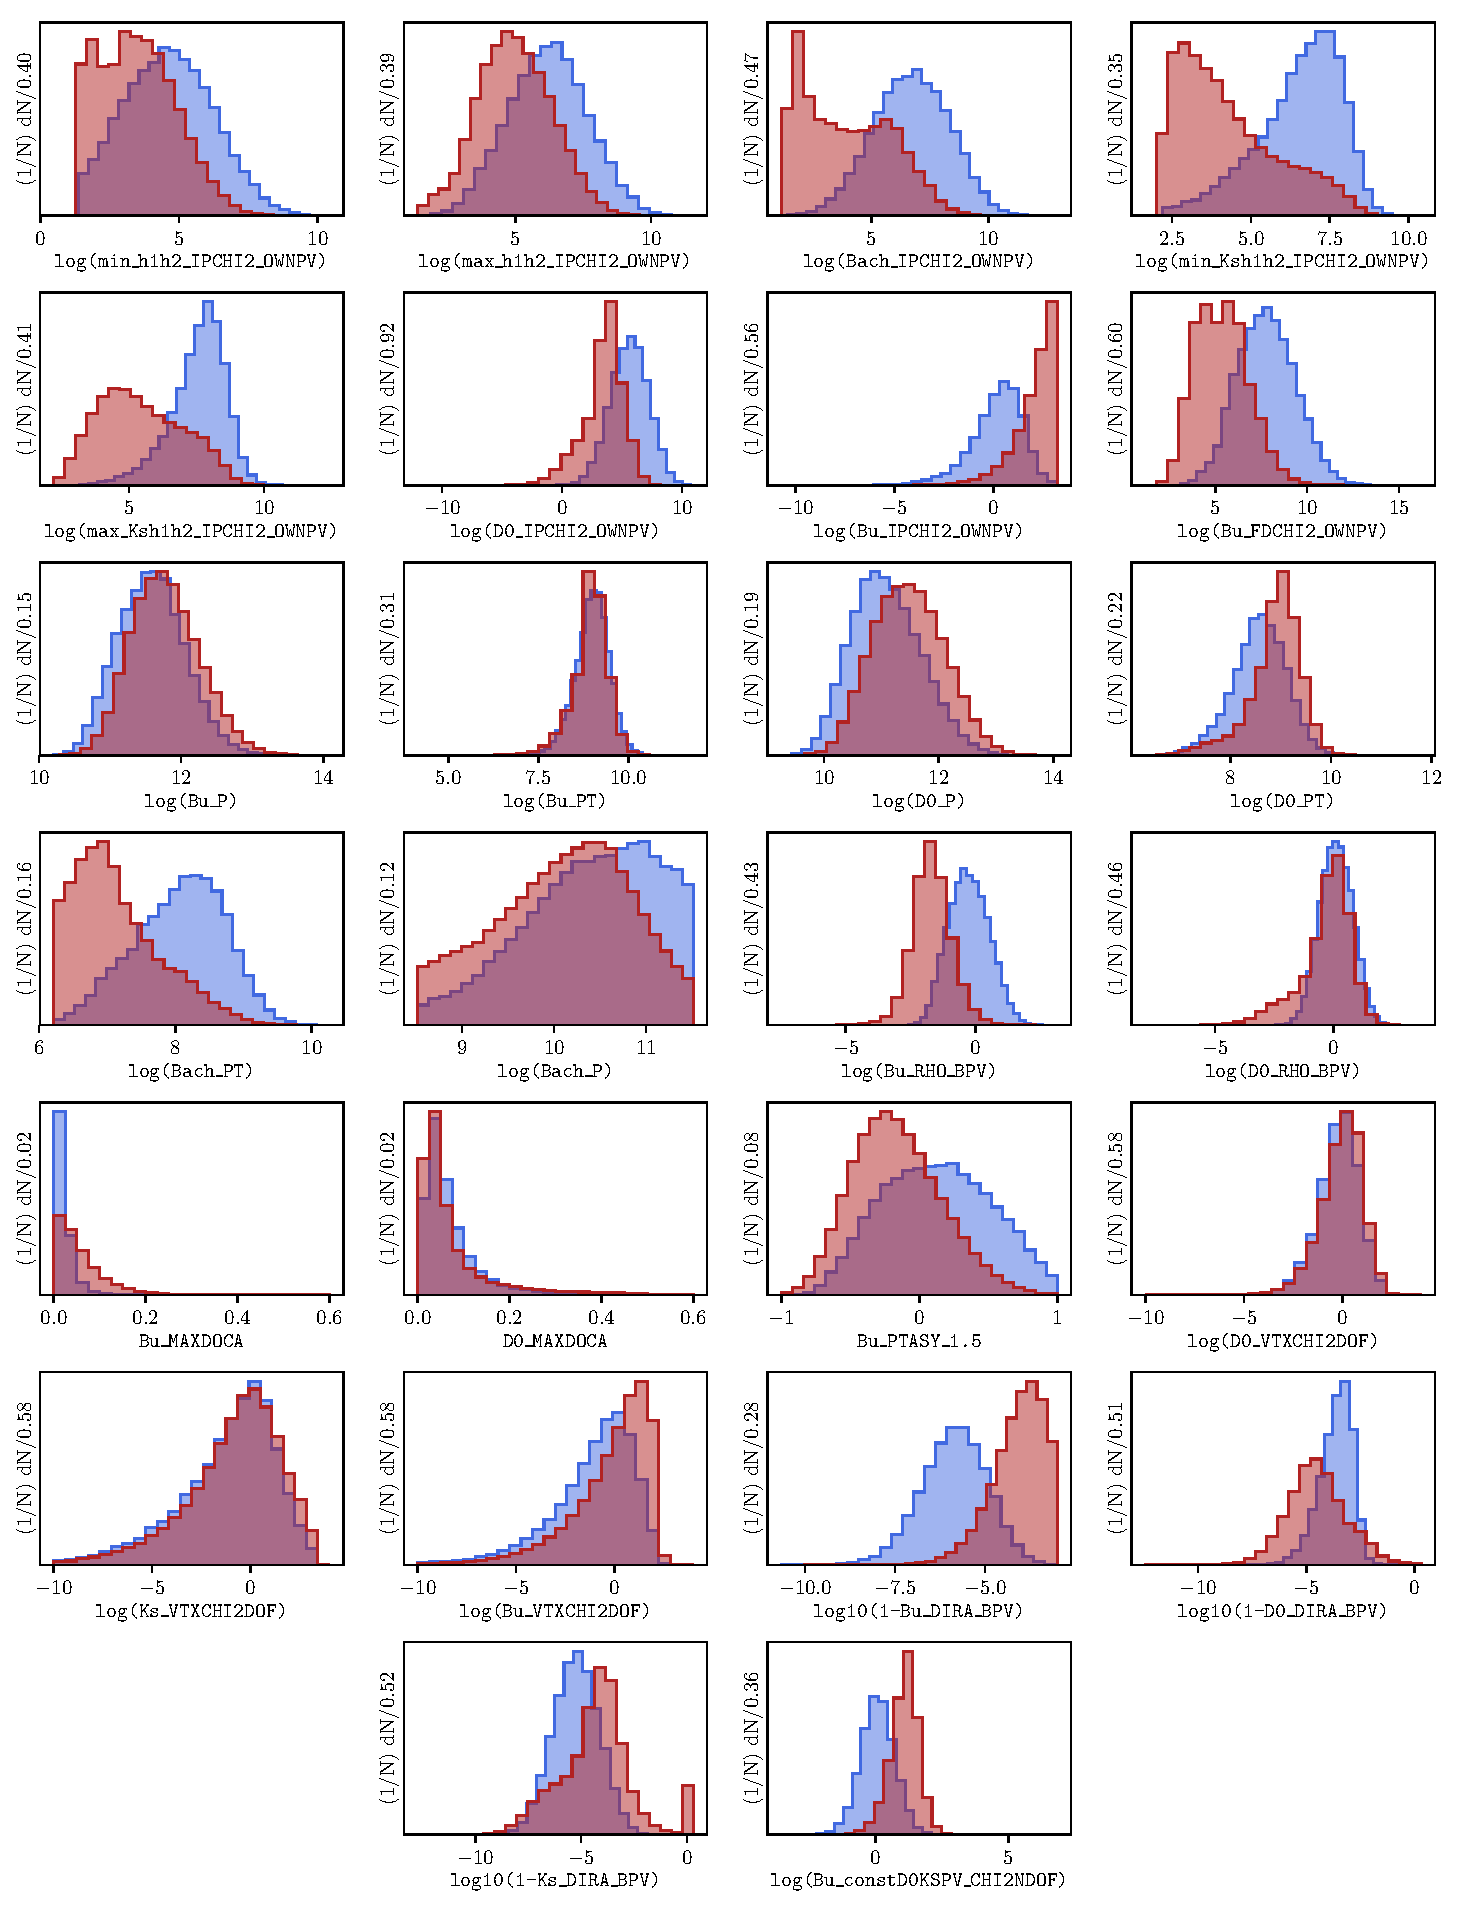
\includegraphics[width=0.95\columnwidth]{figures/analysis/input_param_LL.pdf}
    \caption{Distribution of input parameters in the LL training samples of (blue) signal decays from simulation and (red) background decays from the upper \B sideband. The variable names are defined in Table~\ref{tab:mva_input_parameters}.}
    \label{fig:input_variables_LL}
\end{figure}

\begin{figure}[p!]
    \centering
    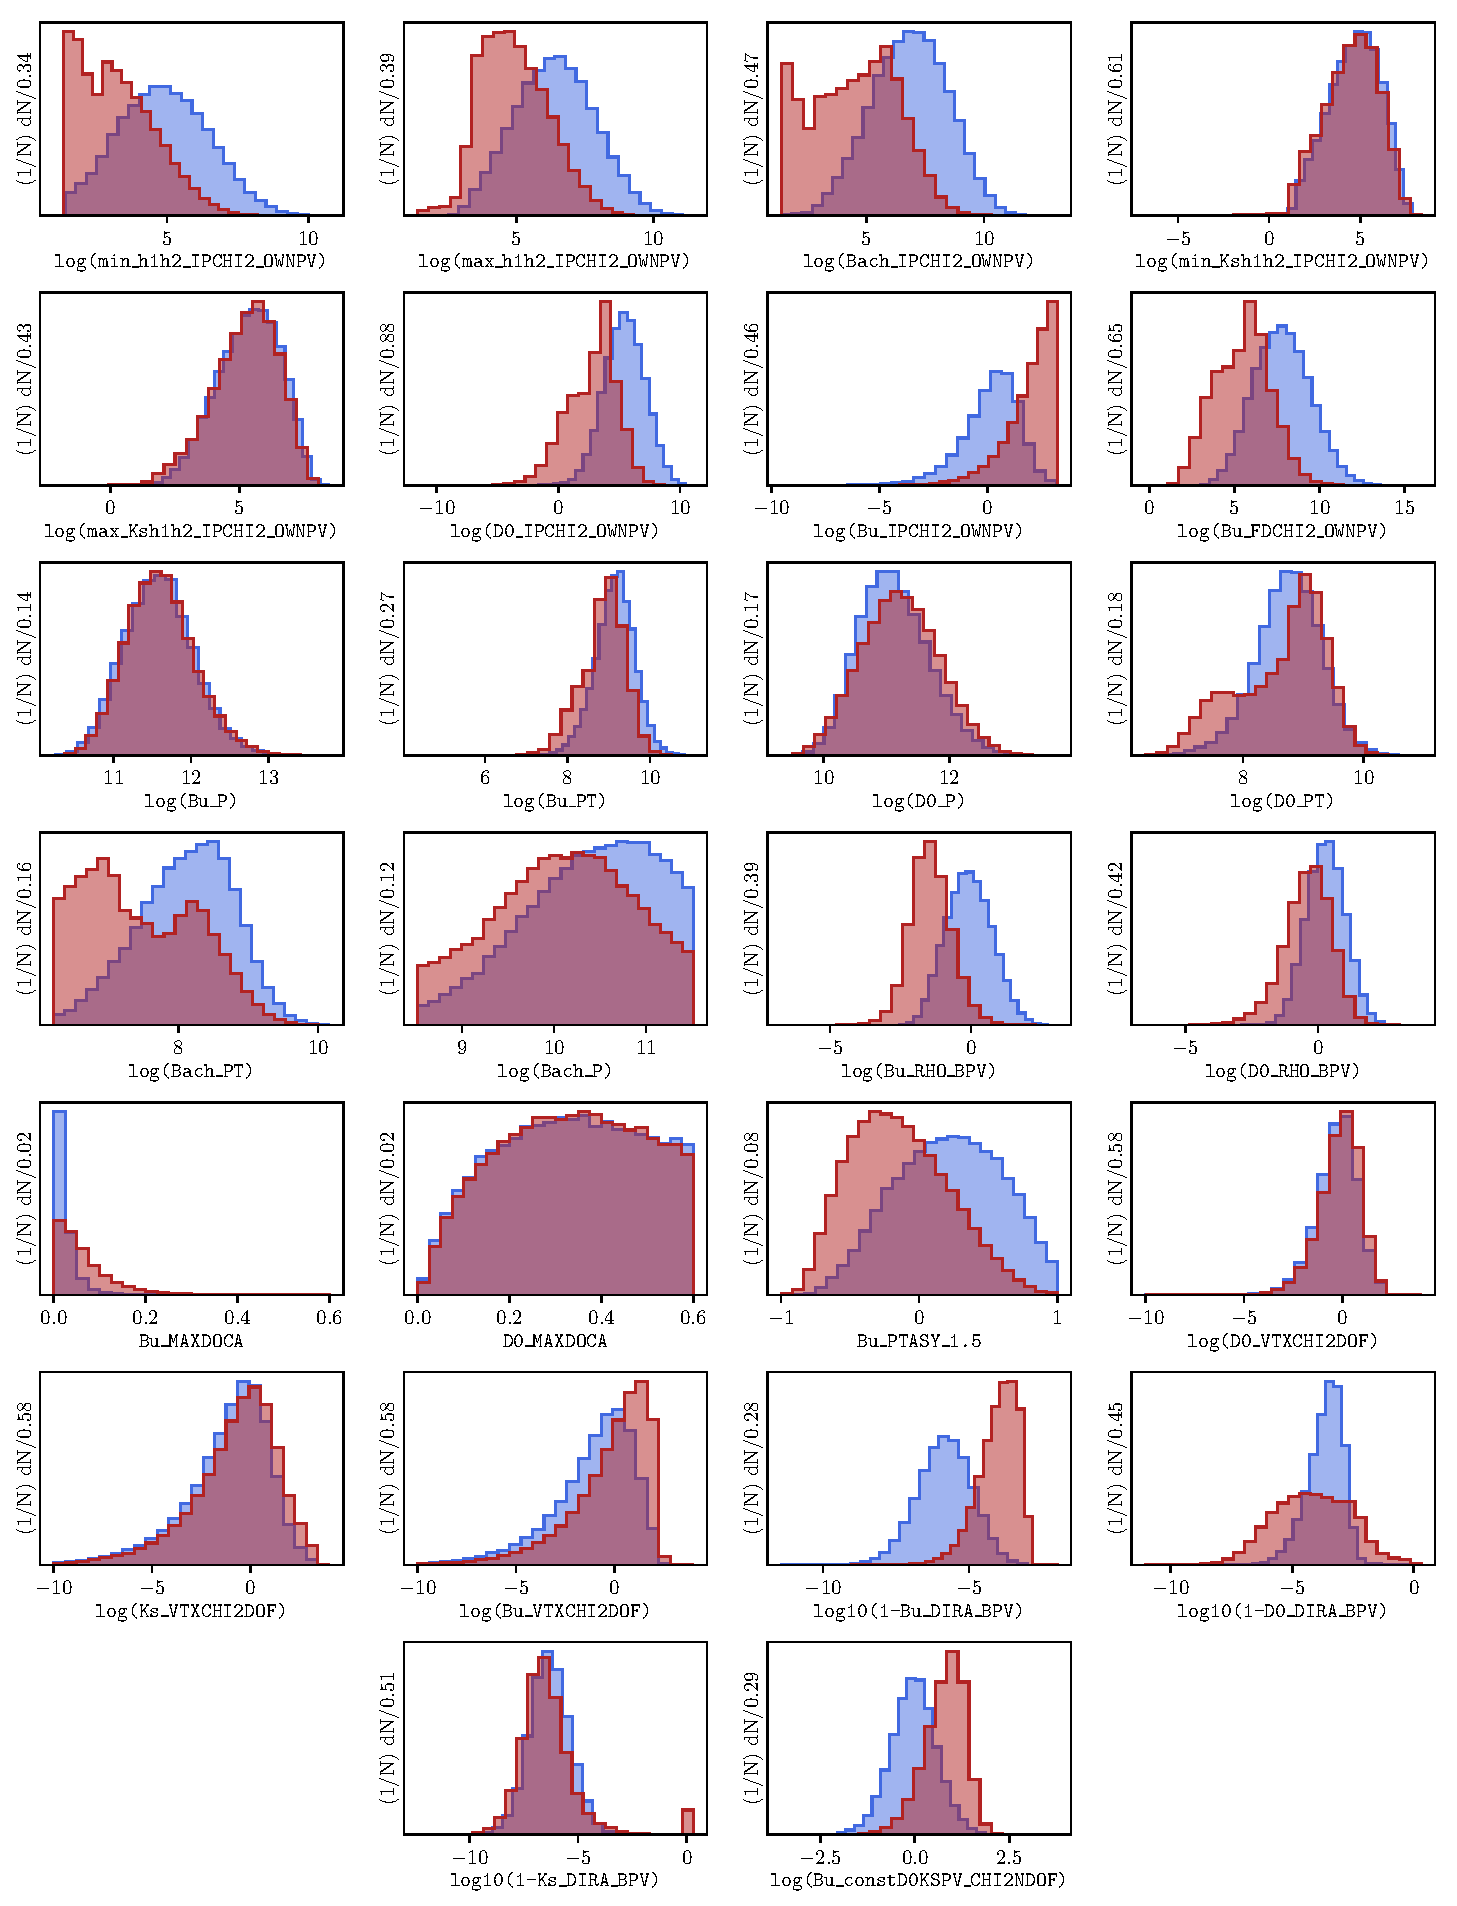
\includegraphics[width=0.95\columnwidth]{figures/analysis/input_param_DD.pdf}
    \caption{Distribution of input parameters in the DD training samples of (blue) signal decays from simulation and (red) background decays from the upper \B sideband. The variable names are defined in Table~\ref{tab:mva_input_parameters}.}
    \label{fig:input_variables_DD}
\end{figure}


The BDTs are trained and tested with input samples representing typical signal and background decay candidates: a signal sample that consists of simulated $\Bpm\to\D(\to\KS\pip\pim)\pipm$ decays corresponding to the \lhcb running conditions for the years 2012--2018, and a sample of combinatorial background candidates from real data, where the reconstructed invariant mass of the \B meson is larger than 5800\mevcc. The candidates in both samples were required to have passed the initial requirements described in the preceding section. The input-parameter distributions in the signal and background training samples are shown in Figs.~\ref{fig:input_variables_LL}~and~\ref{fig:input_variables_DD}. The signal and background samples are each split into two before the training stage: one sub sample, the training sample, is used to train the BDT, after which the trained algorithm is applied to the other sub sample, the test sample. The classifier is found to perform well on the test sample, not just the training sample, which ensures that it does not suffer significant overtraining. The BDT output distribution are shown for both test and training samples in Fig.~\ref{fig:overtrain}, where it is clear that the classifier very effectively separates signal and background candidates.

\begin{figure}[tb]
    \centering
    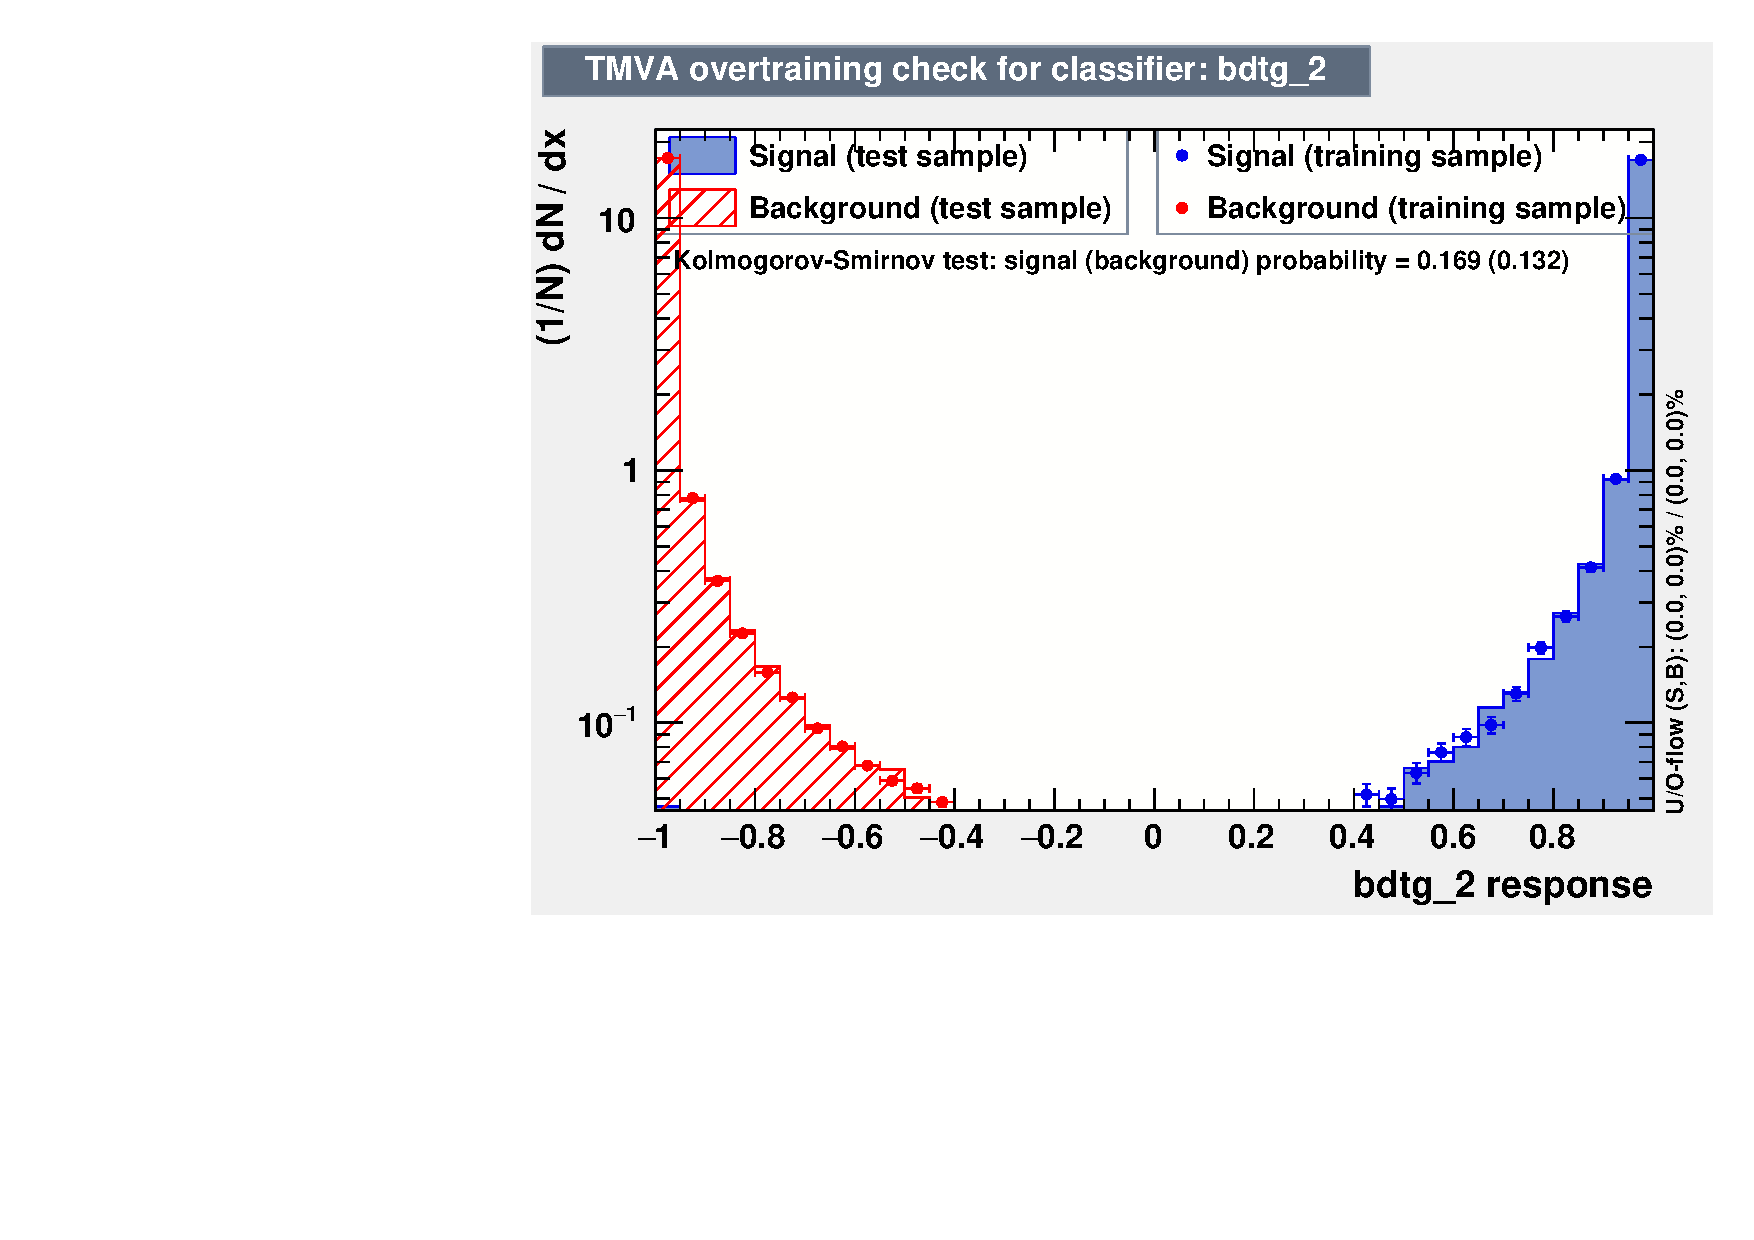
\includegraphics[width=0.45\columnwidth]{figures/analysis/overtrain_check_LL.pdf}
    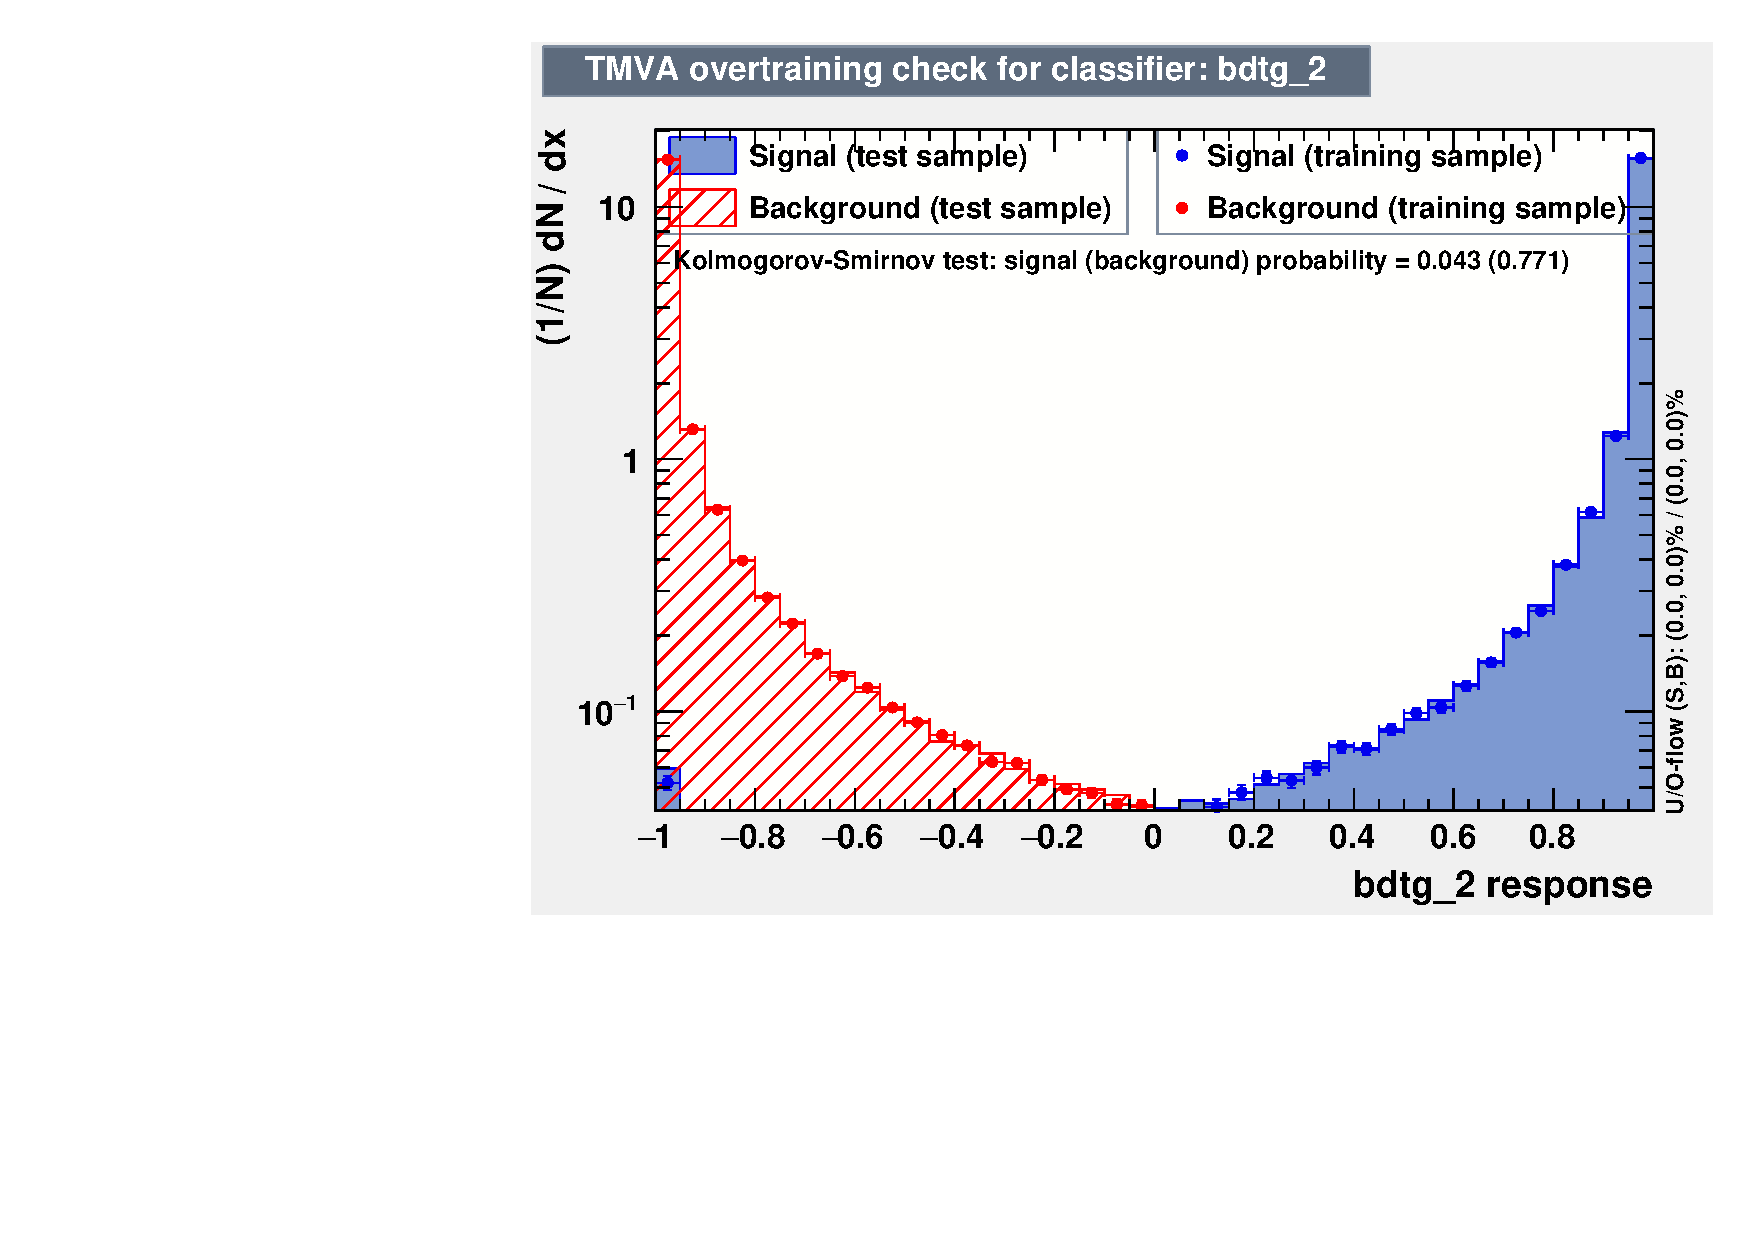
\includegraphics[width=0.45\columnwidth]{figures/analysis/overtrain_check_DD.pdf}
    \caption{Distribution of BDT variable on test and training samples for (left) the LL and (right) the DD category, with logarithmic $y$-scale.}
    \label{fig:overtrain}
\end{figure}

Each candidate in data is classified using the BDT, and candidates that are assigned a score below some threshold value are discarded. The threshold values are chosen in a set of pseudo experiments, such that the expected sensitivity to $\gamma$ is maximised. This is done by performing preliminary fits to the data set for a range of different BDT threshold values, then generating many pseudo data sets with the obtained yields, and applying the full fit and interpretation procedure described in Sections~\ref{sec:signal_and_background_components}--\ref{sec:constraints_on_gamma} to each data set. Thus, the expected uncertainty on $\gamma$ is obtained for for a range of threshold values. The procedure is applied independently for the LL and DD categories, as well as for the Run~1~and~Run~2 data sets, because some parameter distributions differ slightly between the two runs. The optimal threshold values are found to be 0.8 in all situations, except for DD candidates in Run~1 where it is 0.6. This is illustrated in Fig.~\ref{fig:bdt_gamma_scan} where the results of the threshold scans are shown. The same classifier is applied to both \BtoDpi and \BtoDK candidates, and both \D final state categories. While the classifiers were trained using samples of $\Bpm\to\D(\to\KS\pip\pim)\pipm$ simulation and data, the decays are similar enough that no significant improvement in performance was obtained when considering a more elaborate setup. Across all categories, the requirement on the BDT output is found to remove approximately 98\,\% of the combinatorial background, while being approximately 93\,\% efficient on signal.

\begin{figure}[tb]
    \centering
    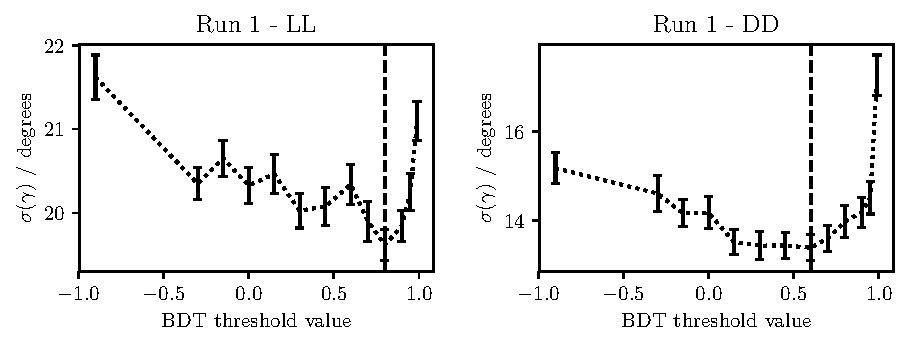
\includegraphics[width=0.85\columnwidth]{figures/analysis/bdt_gamma_scan_Run1_thesis.pdf}
    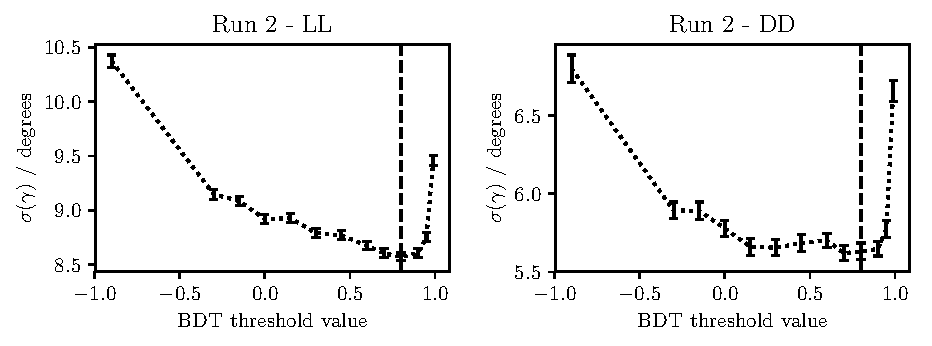
\includegraphics[width=0.85\columnwidth]{figures/analysis/bdt_gamma_scan_Run2_thesis.pdf}
    \caption{The mean uncertainty on $\gamma$ in toy studies, performed with the signal and background yields corresponding to a given BDT requirement, using (top) the Run~1 and (bottom) Run~2 datasets, using only candidates in (left) the LL category and (right) the DD category. The dashed line shows the threshold value employed to discard background-like candidates in the selection.}
    \label{fig:bdt_gamma_scan}
\end{figure}
% subsection boosted_decision_tree (end)


\subsection{Particle-identification requirements} % (fold)
\label{sub:particle_identification_requirements}

A PID requirement is made to separate \BtoDK and \BtoDpi candidates in the data sample, by requiring that the \texttt{PIDK} of the companion particle satisfies $\texttt{PIDK} < 4$ for \BtoDpi candidates and $\texttt{PIDK} > 4$ for \BtoDK candidates. The \texttt{PIDK} variable was defined in Section~\ref{sub:the_rich}. This ensures that any given candidate is selected into only one of these samples.

Further to the requirement on the companion, PID requirements are made to suppress semi-leptonic backgrounds as well as decays where a final state particle decays in flight, and a loose PID requirement is made in the $\D\to\KS\Kp\Km$ channels where it leads to a higher signal purity:
\begin{itemize}
    \item the companion particle is required to satisfy $\texttt{IsMuon}=0$.
    \item For the $\B\to\D(\to\KS\pip\pim)h^{\pm}$ samples it is require that the charged pion track from the \D decay with opposite charge to the companion satisfies ${\texttt{PIDe} < 0 \;\&\; \texttt{IsMuon}=0}$, and for the other charged pion that ${\texttt{IsMuon}=0}$. A very loose requirement of $\texttt{PIDK} < 20$ is applied to both pions from the \D-decay in the stripping stage.
    \item For the $\B\to\D(\to\KS\Kp\Km)h^{\pm}$ samples it is required that the charged kaon tracks from the \D decay have RICH information, a momentum less than 100 \gevc and ${\texttt{PIDK} > -5 \;\&\; \texttt{IsMuon}=0}$.
\end{itemize}
These backgrounds are described in Section~\ref{sub:semi_leptonic_backgrounds}.


% subsection particle_identification_and_final_requirements (end)

\subsection{Final requirements} % (fold)
\label{sub:final_requirements}

For a small fraction of candidates in the final sample, it is the case that two or more candidates originate in the same $pp$ collision. In order to make sure that all candidates are completely independent, a single, arbitrary candidate from each $pp$ collision is kept for these collisions, and the other candidates discarded. This requirements results in the removal of less than 0.7\,\% of candidates in each data category.

Furthermore, the \D mass used to define the binning schemes described in Ref.~\cite{CLEOCISI} differs slightly from the mass used in the DTF refit. Therefore a few of the decays are reconstructed with Dalitz coordinates outside the allowed kinematic region. This problem concerns less than 0.5\,\% (1\,\%) of candidates in the \DtoKspp (\DtoKskk) channel and they are simply discarded. The \BtoDK and \BtoDpi channels are equally affected, and therefore the effect is inherently taken into account in the analysis, similarly to other phase-space-dependent acceptance effects.

% subsection final_requirements (end)

\subsection{Selected candidates} % (fold)
\label{sub:selected_candidates}

\begin{table}[tbp]
    \centering
    \caption{Final candidate yield in each data category after the full selection has been applied, including removing candidates outside the region $m_B\in [5080, 5800]\mevcc$.}
    \label{tab:final_data_candidate_yields}
    % \scriptsize
    \begin{tabular}{lll|ccc}
        \hline
        \hline
        \B Decay & \D final state& \KS type &  Run 1 & Run 2 & Total\\

        \hline
        \BtoDK & \Kspipi     &LL   
        & {2275} & {10525} & {12800}\ \\
               &             &DD   
        & {5097} & {23508} & {28605}\\
               & \KsKK       &LL   
        & {383} & {1610} & {1993}\  \\
               &             &DD   
        & {772} & {3397} & {4169}\\
        \hline
        \BtoDpi & \Kspipi    & LL  
        & {18209} & {90509} & {108718}\\
                &            & DD  
        & {40167} & {205807} & {245974} \\
                & \KsKK      & LL  
        & {2879} & {13757} & {16636}\ \\
                &             & DD  
        & {6033} & {29790} & {35823}\\
        \hline\hline       
    \end{tabular}
\end{table}

\begin{figure}[tbp]
    \centering
    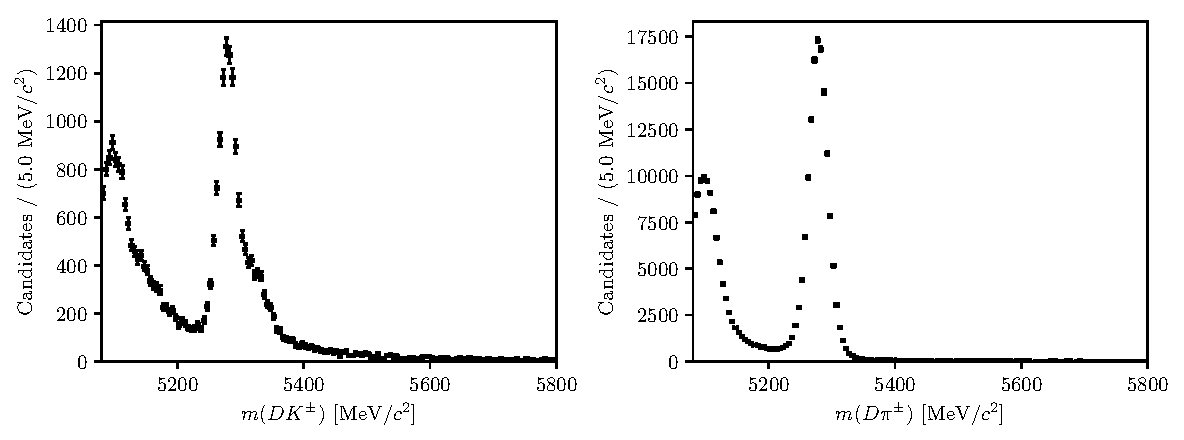
\includegraphics[width=\columnwidth]{figures/analysis/pretty_data_d2kspp_DD.pdf}
    \caption{The spectrum of $m_B$ in the (left) \BtoDK and (right) \BtoDpi samples where \DtoKspipi and the \KS meson is reconstructed in the DD category, after the full selection has been applied.}
    \label{fig:data_spectrum}
\end{figure}

In total, about 47,000 \BtoDK candidates and 400,000 \BtoDpi candidates are selected, as summarised in Table~\ref{tab:final_data_candidate_yields}. An example of the \B mass distribution in one of the data categories is shown in Fig.~\ref{fig:data_spectrum}; it is clear that a significant number of these candidates are background decays. The Dalitz plots for candidates in the signal region where $m_B\in[5249, 5309]\mevcc$ are shown in Fig.~\ref{fig:dalitz_plots_KsPiPi}~and~\ref{fig:dalitz_plots_KsKK}. Due to the large yields in the full Run~1~and~2 \lhcb data set, the asymmetries between the \Bp and \Bm distributions are visible to the eye in the \BtoDK plots.

\begin{figure}[tp]
    \centering
    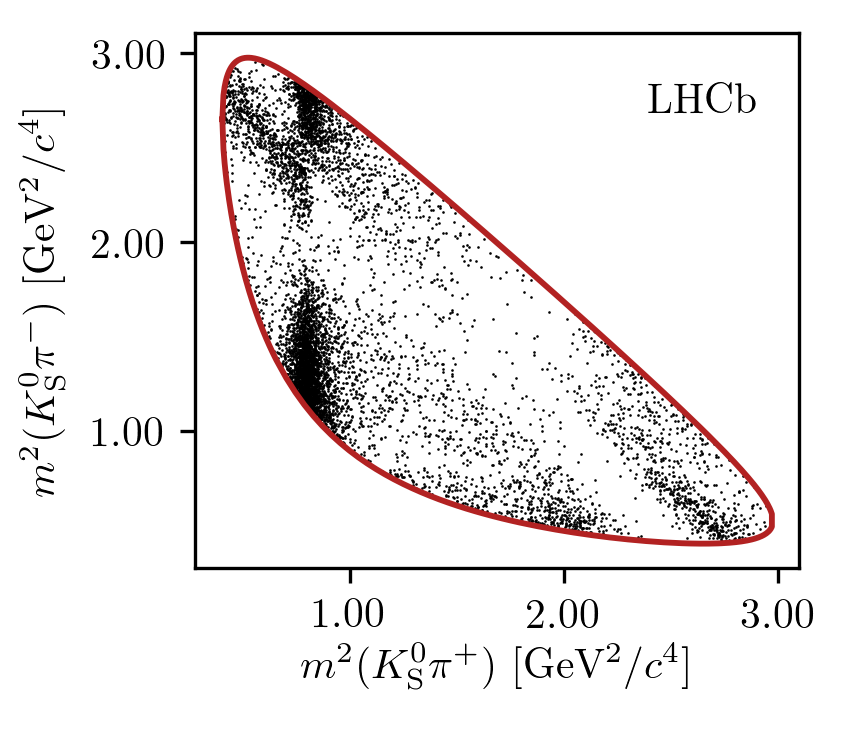
\includegraphics[width=0.45\columnwidth]{figures/analysis/dalitz_plots/single_DP_K_PiPi_LLandDD_plus.png}
    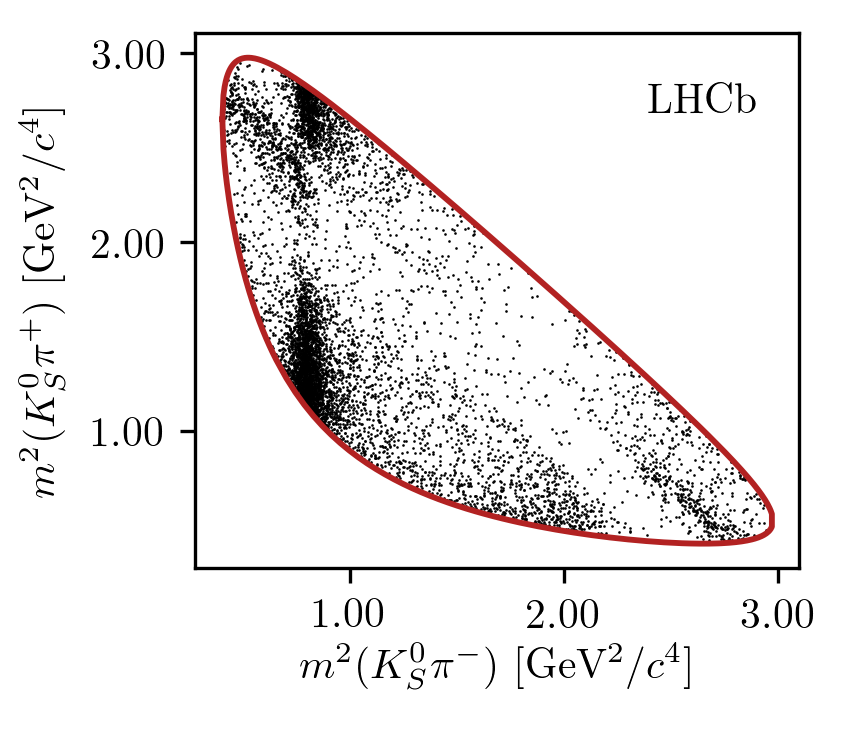
\includegraphics[width=0.45\columnwidth]{figures/analysis/dalitz_plots/single_DP_K_PiPi_LLandDD_minus.png}
    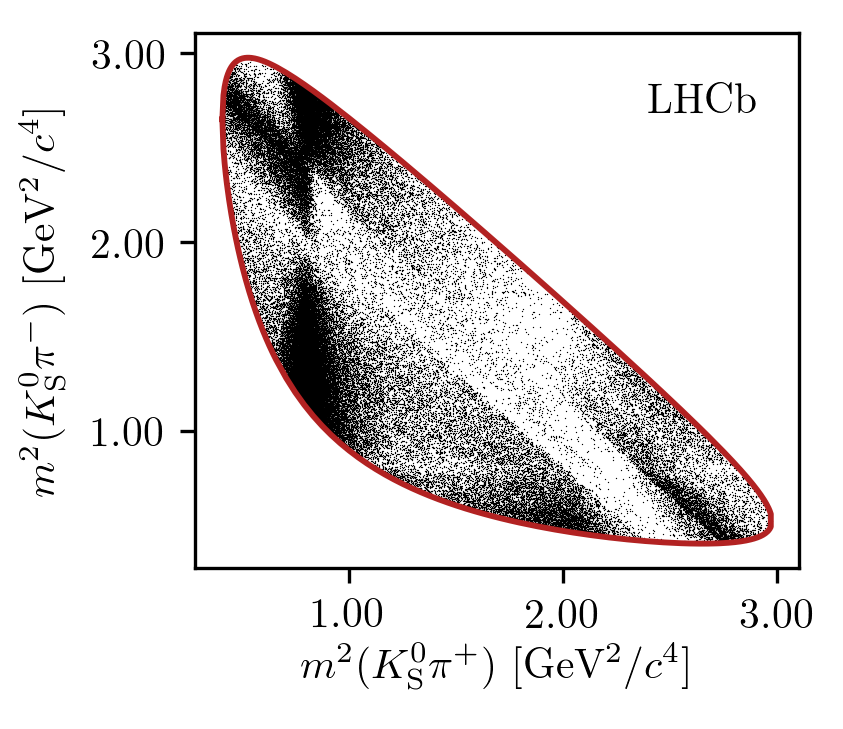
\includegraphics[width=0.45\columnwidth]{figures/analysis/dalitz_plots/single_DP_Pi_PiPi_LLandDD_plus.png}
    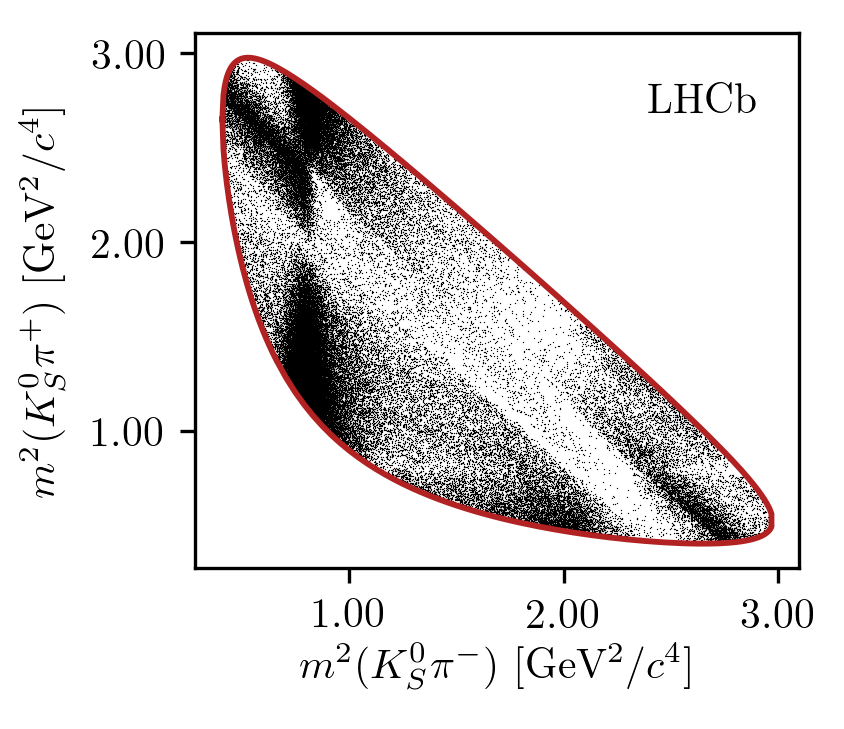
\includegraphics[width=0.45\columnwidth]{figures/analysis/dalitz_plots/single_DP_Pi_PiPi_LLandDD_minus.png}
    \caption{Dalitz plots of (left) $\Bp\to\D h^+$ and (right) $\Bm\to\D h^-$ candidates in the signal region, in the (top) \BtoDK and (bottom) \BtoDpi channels where \DtoKspipi. The LL and DD categories have been combined.}
    \label{fig:dalitz_plots_KsPiPi}
\end{figure}

\begin{figure}[tp]
    \centering
    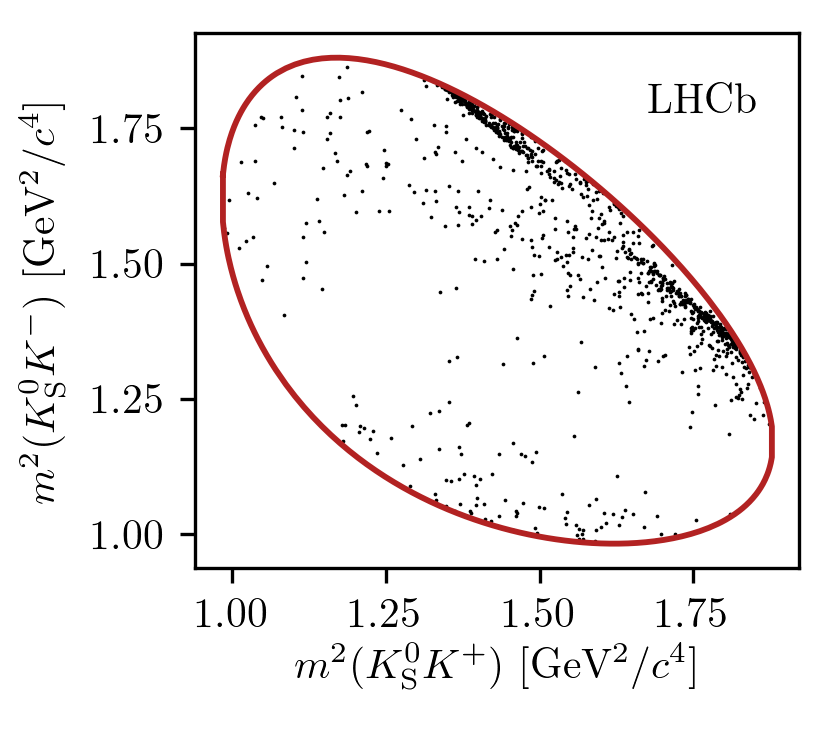
\includegraphics[width=0.45\columnwidth]{figures/analysis/dalitz_plots/single_DP_K_KK_LLandDD_plus.png}
    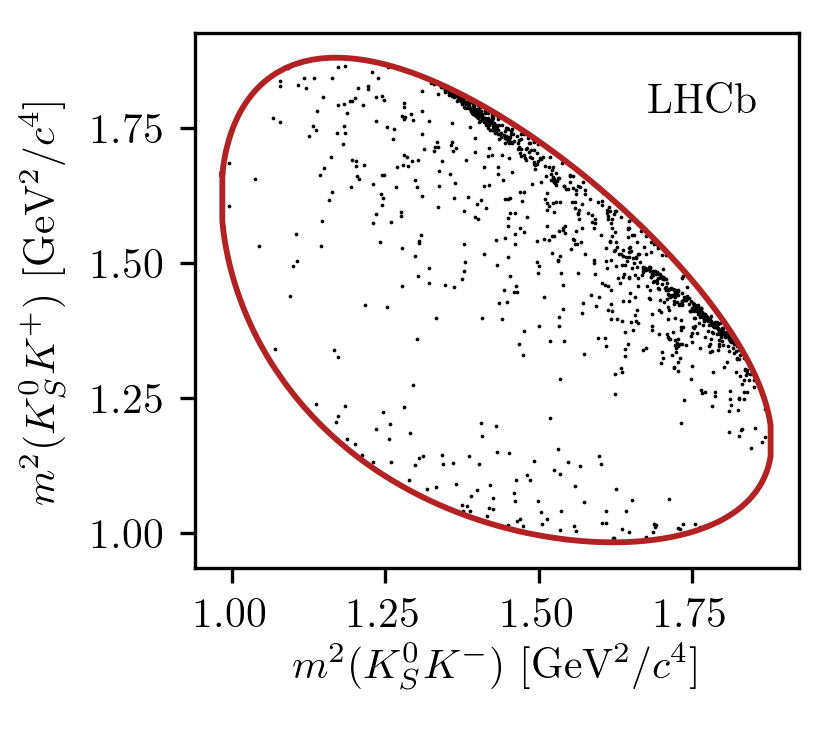
\includegraphics[width=0.45\columnwidth]{figures/analysis/dalitz_plots/single_DP_K_KK_LLandDD_minus.png}
    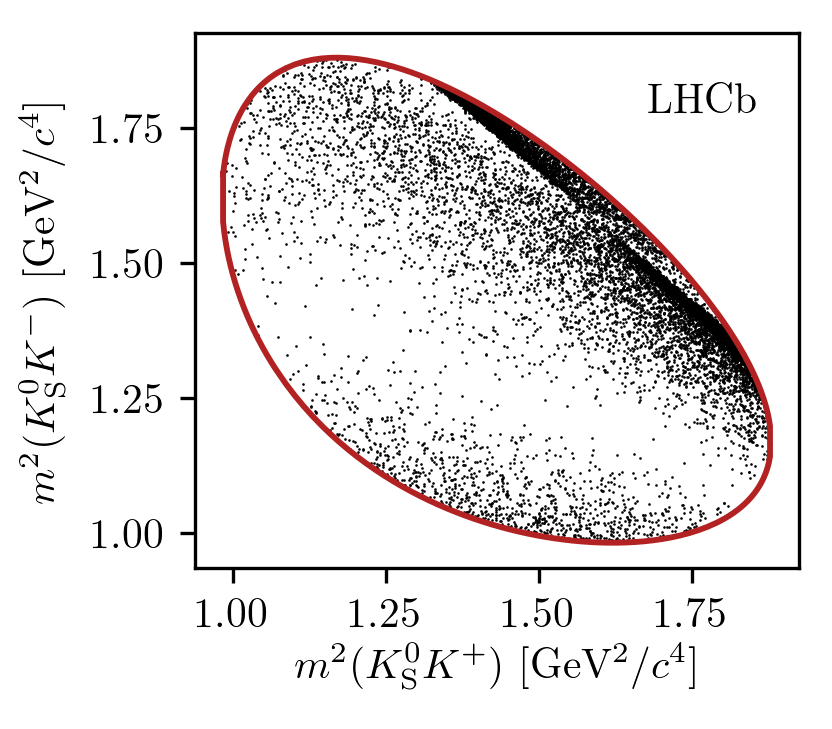
\includegraphics[width=0.45\columnwidth]{figures/analysis/dalitz_plots/single_DP_Pi_KK_LLandDD_plus.png}
    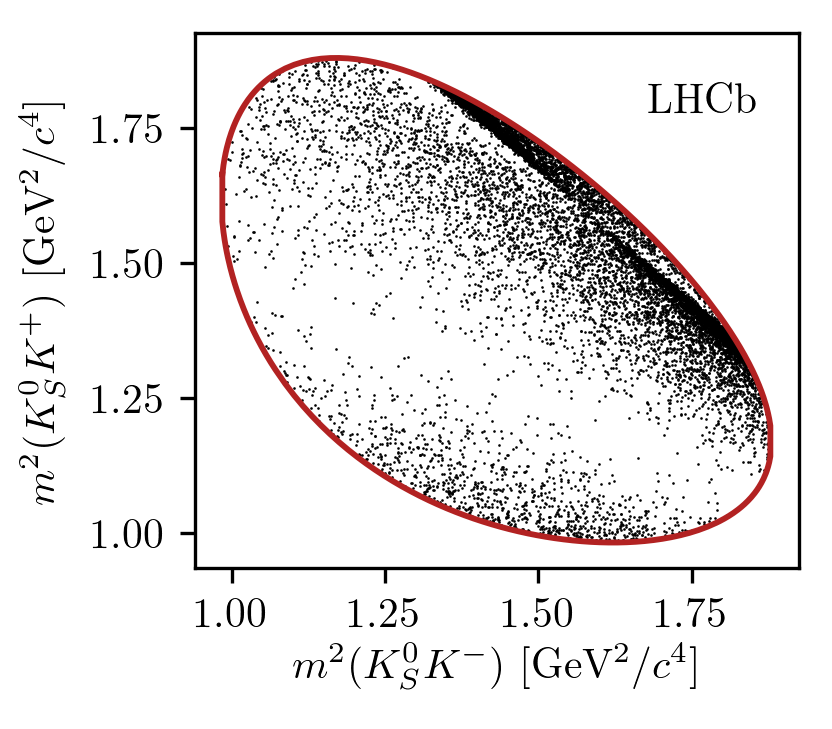
\includegraphics[width=0.45\columnwidth]{figures/analysis/dalitz_plots/single_DP_Pi_KK_LLandDD_minus.png}
    \caption{Dalitz plots of (left) $\Bp\to\D h^+$ and (right) $\Bm\to\D h^-$ candidates in the signal region, in the (top) \BtoDK and (bottom) \BtoDpi channels where \DtoKsKK. The LL and DD categories have been combined.}
    \label{fig:dalitz_plots_KsKK}
\end{figure}

% subsection selected_candidates (end)

% section candidate_selection (end)
\FloatBarrier
\section{Signal selection efficiencies} % (fold)
\label{sec:signal_selection_efficiencies}

% 2) The efficiency study needs to go somewhere. You refer to it in Sec[??] but that section doesn’t exist. My suggestion would be after the selection have an extra section where you discuss the similarity of the Dpi and DK selection in simulation and show the plots of the 3 DP variables and the 2D plot, and the fit to show that the division is modelled well by a flat line .

% This is not a lot of work.

% To that section i think you could also add a small additional amount of information on the selection. What i’m thinking of is the various efficiencies of the various cuts on the signal MC. You have nice plots in the ANA already so with just a small modification these would be ready quickly. I think it is important that you convey to the reader how much singal is lost by the various cuts that are applied (base, charmless, ks, pid, bdt). At the moment you only comment on the BDT, and PID. Addition of plots that would give the indication for the base cuts and other physics backgrounds would be a good addition.
% If you have some unbuggy MC then another thing to add would be an indication of the overall efficiency - doesn’t need to be detailed of more accurate than a single number in a sentence. 

The efficiency of each step of the selection on signal decays can be investigated using simulated decays. In the \BtoDpi channel, only decays that were placed in the "test" sample when training the BDT are used, in order to avoid overestimating the efficiency. 

In general, the total selection efficiency up until the PID requirements, including the offline stage and the effect of the geometrical \lhcb acceptance, is about 1 permille, slightly higher for \BtoDK than \BtoDpi decays, slightly higher for \DtoKsKK than \DtoKspipi decays, and somewhat higher in the Run~2 than in Run~1 due to improvements in the trigger. The PID requirements are investigated separately in Section~\ref{sub:efficiency_of_the_pid_requirements} below, using samples of calibration data. The overall selection efficiency does not impact the measurement at all, because the observables of interest are sensitive  \emph{only} to the distribution of decays over the Dalitz plot (except, of course, in the sense that a higher signal efficiency is desirable because it leads to larger signal yields). Likewise, it makes no difference that the overall selection efficiencies differ slightly between \BtoDK and \BtoDpi decays, as long as the efficiency profile over the Dalitz plot is identical between the two decay channels. This is confirmed separately in Section~\ref{sub:efficiency_profile_over_the_dalitz_plot} below.

\begin{figure}[tp]
    \centering
    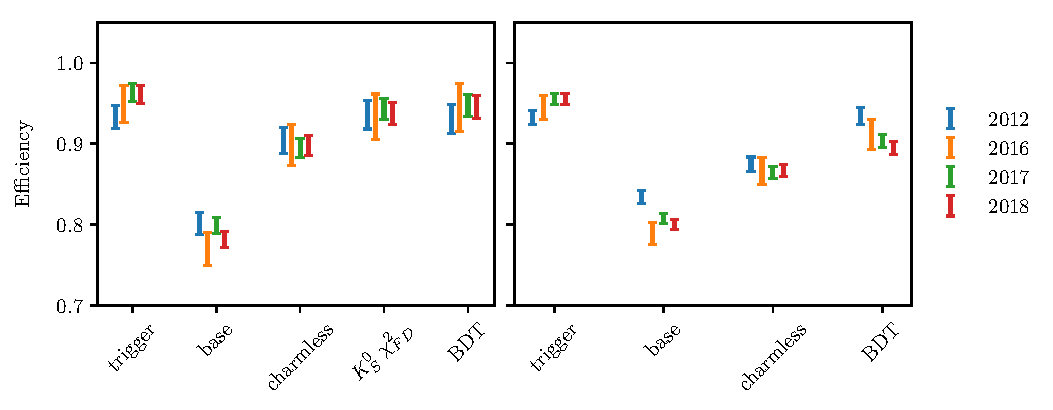
\includegraphics[width=0.98\columnwidth]{figures/analysis//relative_cutflow_signal_thesis.pdf}
    \caption{The efficiency of each selection step in samples of simulated ${\Bpm\to\D(\to\KS\pip\pim)\pipm}$ signal decays in the (left) LL and (right) DD categories. The selection steps are applied on top of each other, from left to right on the horizontal axis. The samples are split by year. }
    \label{fig:sig_rel_cutflow}
\end{figure}



The efficiencies of each individual selection step are shown in Fig.~\ref{fig:sig_rel_cutflow}, obtained using simulated \BtoDpi decays. The main reason that some signal decays do not survive the base requirement is the ${p_\mathrm{companion}<100\gevc}$ requirement, which is in place to ensure that the PID performance for the companion is good. For decays with $p_\mathrm{companion}>100\gevc$, only about $60\,\%$ of \BtoDK decays survive the subsequent $\texttt{PIDK}>4$ requirement and the cross-feed from misidentified \BtoDpi decays is $50\,\%$ larger than in the current selection. Thus, loosening this requirement leads to little statistical gain, while leading to larger systematic effects from the crossfeed background.


\begin{figure}[tp]
    \centering
    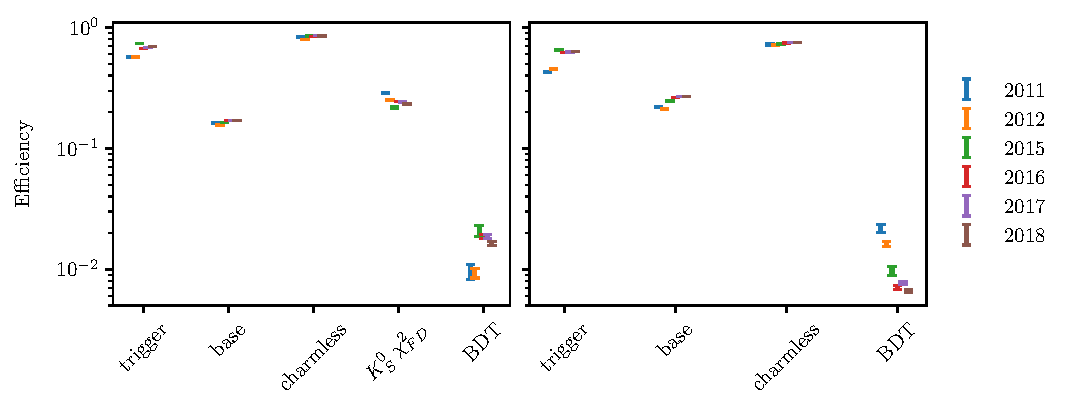
\includegraphics[width=0.98\columnwidth]{figures/analysis/relative_cutflow_combinatorial_thesis.pdf}
    \caption{
    The efficiency of each selection step in samples of ${\Bpm\to\D(\to\KS\pip\pim)\pipm}$ candidates in data where the reconstructed \B mass is above 5600\mevcc, meaning the candidates stem from combinatorial background. The efficiency is shown for candidates in the (left) LL and (right) DD categories. The selection steps are applied on top of each other, from left to right on the horizontal axis. The samples are split by year. Notice the logarithmic scale on the vertical axis.}
    \label{fig:comb_rel_cutflow}
\end{figure}

An equivalent plot for the combinatorial background  is shown in Fig.~\ref{fig:comb_rel_cutflow}, using $\Bpm\to\D(\to\KS\pip\pim)\pipm$ candidates in data with a reconstructed \B mass above $5600\mevcc$; it can be seen that the BDT is very efficient at rejecting combinatorial background, but that the base requirements and the requirement on the \KS flight distance also remove a decent amount of background.



\subsection{Efficiency of the PID requirements} % (fold)
\label{sub:efficiency_of_the_pid_requirements}

The efficiencies of the PID requirements on the companion enter the yield parameterisations of the mass fits in Section~\ref{sec:signal_and_background_components}~and ~\ref{sec:measurement_of_the_cp_violation_observables} and must therefore be known. They are determined using samples of calibration data selected without relying on PID variables, as implemented in the $\texttt{PIDCalib}$ frame work~\cite{anderliniPIDCalibPackage2016}. Reasonably pure samples of pion and kaon tracks are obtained from $\Dz\to\Km\pip$ decays, where the \D meson originates in a $\Dstarp\to\Dz\pip$ decay and can therefore be flavour tagged. The remaining background is subtracted via the \emph{sPlot}~\cite{sPlot} procedure, based on a two-dimensional fit of the $m(\Km\pip)$ and $m(\Dz\pip)-m(\Dz)$ distributions. The obtained weights are employed to calculate the average efficiency of the requirement on $\texttt{PIDK}$ for a number of bins in the momentum and pseudorapidity of the calibration tracks, and the number of charged tracks in the detector, thus constructing a three-dimensional efficiency lookup table. The procedure is carried out for each PID requirement, companion species, data-taking year, track charge, and magnet polarity. Based on these tables, expected PID efficiencies for the \BtoDpi and \BtoDK signal decays are calculated that take the kinematical distribution and detector occupancy in the BPGGSZ data samples into account, by using the high-purity sample of \BtoDpi candidates in the signal region as a reference. The dominating uncertainty on the efficiencies is statistical in nature, due to the finite size of the reference sample. In addition, systematic uncertainties are included due to the sPlot procedure, estimated at $0.1\,\%$~\cite{anderliniPIDCalibPackage2016}, and due to the choice of binning scheme, estimated by repeating the procedure using a number of alternative binning schemes. The final estimates of the correct-ID efficiencies, $\varepsilon_\text{PID}$, are shown in Table~\ref{tab:PIDeffs}, including all sources of uncertainty. Note that the probability to misidentify a decay satisfies $\varepsilon_\text{mis-ID}=1-\varepsilon_\text{PID}$ by construction, due to the the definition of the \texttt{PIDK} variable (given in Section~\ref{sub:particle_identification}) and the chosen PID requirement.

% autogenerated by ANA_scripts/03_selection/efficiency_studies/PIDEfficiencyCalculations.ipybn
% 2019-10-23 14:18:35.597522

\def \pidEffPitoPiDtoPiPiLL {$ 97.11 \pm 0.11$}
\def \pidEffPitoPiDtoPiPiDD {$ 97.17 \pm 0.13$}
\def \pidEffPitoPiDtoKKLL {$ 97.07 \pm 0.11$}
\def \pidEffPitoPiDtoKKDD {$ 97.16 \pm 0.14$}
\def \pidEffKtoKDtoPiPiLL {$ 86.74 \pm 0.13$}
\def \pidEffKtoKDtoPiPiDD {$ 86.90 \pm 0.22$}
\def \pidEffKtoKDtoKKLL {$ 86.22 \pm 0.26$}
\def \pidEffKtoKDtoKKDD {$ 86.56 \pm 0.30$}


\begin{table}[tb]
\centering
\caption{PID efficiencies obtained with the \texttt{PIDCalib} tool. The uncertainty incorporates statistical uncertainty due to the size of the reference sample, the systematic uncertainty due to the choice of binning scheme in \texttt{PIDCalib}, and a systematic uncertainty due to the \texttt{sWeight} calculation in \texttt{PIDCalib} of $0.1\,\%$.
\label{tab:PIDeffs}}
\begin{tabular}{l l l c c}
\hline\hline
Efficiency & Particle & \D final state & \multicolumn{2}{c}{$\varepsilon_{\text{PID}}\,(\%)$} \\
\cline{4-5}     
           &      &             & LL                        & DD                \\
\hline  
\multicolumn{5}{c}{Run I and II}\\
\hline  
Correct ID & Kaon & \DtoKspp    & \pidEffKtoKDtoPiPiLL      & \pidEffKtoKDtoPiPiDD     \\
           &      & \DtoKskk    & \pidEffKtoKDtoKKLL        & \pidEffKtoKDtoKKDD       \\
           & Pion & \DtoKspp    & \pidEffPitoPiDtoPiPiLL    & \pidEffPitoPiDtoPiPiDD   \\
           &      & \DtoKskk    & \pidEffPitoPiDtoKKLL      & \pidEffPitoPiDtoKKDD     \\
\hline\hline
\end{tabular}
\end{table}

% subsection efficiency_of_the_pid_requirements (end)

\subsection{Efficiency profile over the Dalitz plot} % (fold)
\label{sub:efficiency_profile_over_the_dalitz_plot}



The analysis strategy depends on sharing the $F_i$ parameters between the $\B\to\D\pi$ and $\B\to\D\kaon$ channels. This is reasonable, since the phase-space dependence of the reconstruction efficiency is expected to be very similar between the two decays, given the similar kinematics; an assumption that is verified using samples of simulated decays. The full selection is applied to the samples. The $\B\to\D\pi$ sample of LL (DD) candidates includes about 63,000 (146,000) simulated decays, and the $\B\to\D\kaon$ samples include 60,000 (142,000) simulated decays. For the $\B\to\D\pi$ mode, this is approximately equal to the number of decays in the full Run~1+2 data sample, and for $\B\to\D\kaon$ this is a factor of about 12 larger than the data sample. The decays were simulated with an equal decay probability across the \D-decay phase space, so that any non-uniform distribution of reconstructed decays is completely determined by a phase-space dependent reconstruction and selection efficiency. Therefore the assumption that the phase-space dependence is identical between the $\B\to\D\pi$ and $\B\to\D\kaon$ channels is verified by seeing if the Dalitz coordinates are distributed differently between the samples of simulated $\B\to\D\pi$ and $\B\to\D\kaon$ decays.

\begin{figure}[tbp]
    \centering
    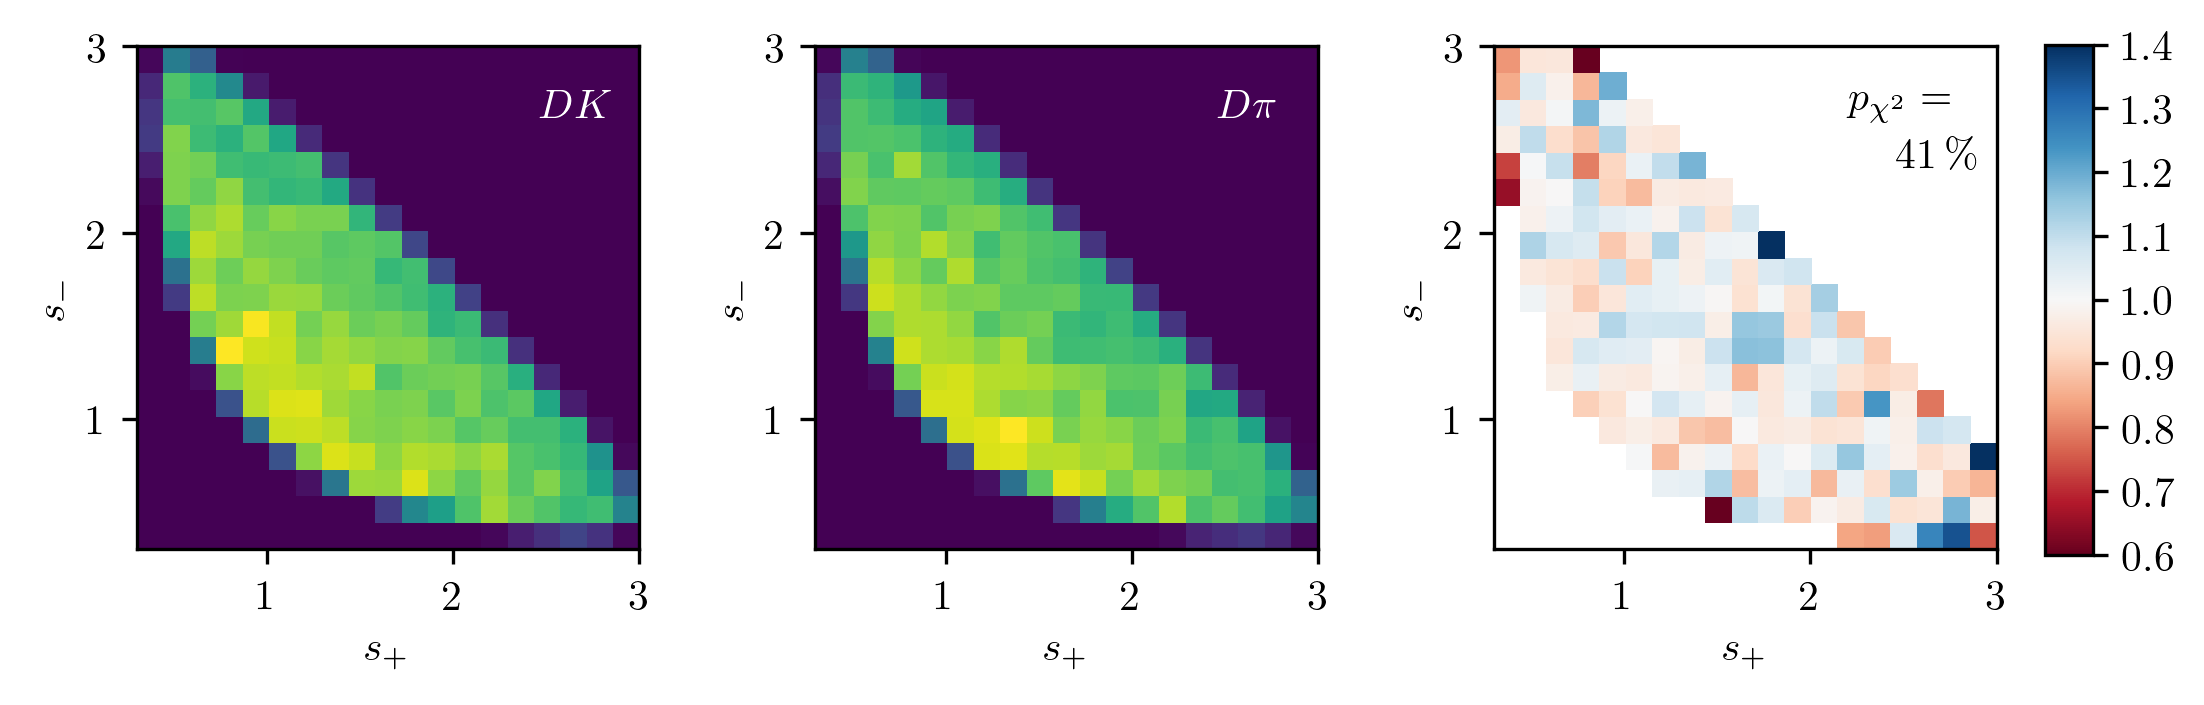
\includegraphics[width=\columnwidth]{figures/analysis/DP_thesis_m2_chi2_PiPi_LL.png}
    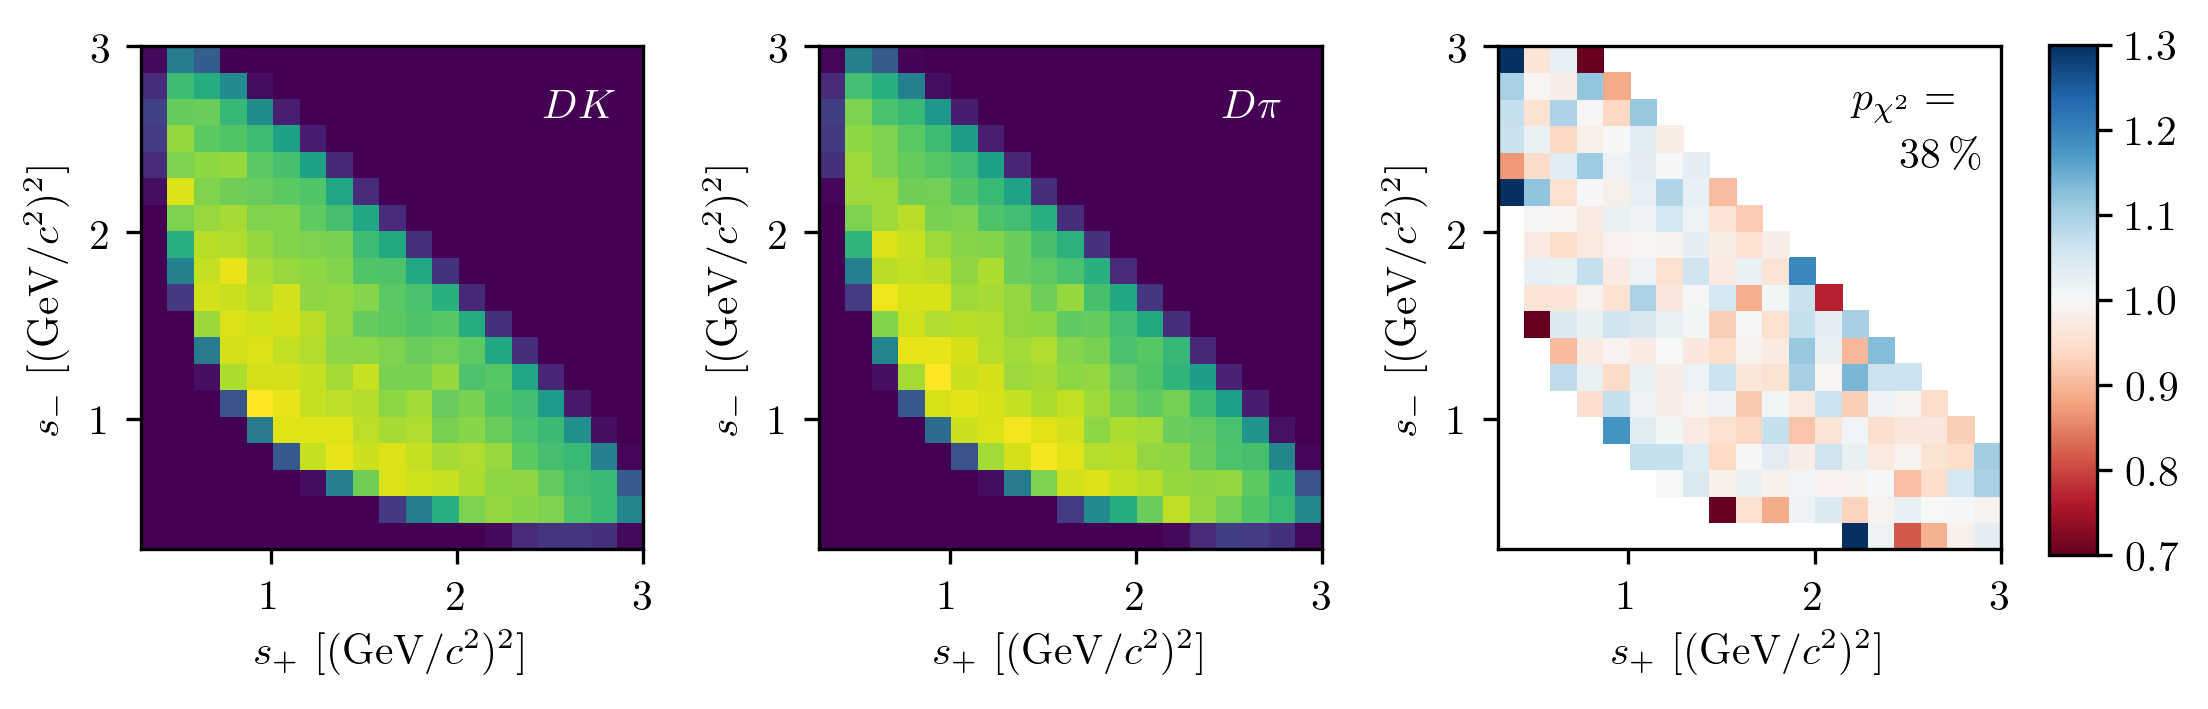
\includegraphics[width=\columnwidth]{figures/analysis/DP_thesis_m2_chi2_PiPi_DD.png}
    \caption{The $(s_+, s_-)$ distribution in simulated samples of (left)  $\B\to\D\kaon$ decays and (center)  $\B\to\D\pi$ decays where \DtoKspipi, as well as (right) the ratio between the two histograms (corrected for differences in sample sizes). The plots are shown for for candidates in the (top) LL and (bottom) DD categories. The $p$ values are the results of $\chi^2$ compatibility tests between the two histograms.}
    \label{fig:dk_vs_dpi_chi2_pipi}
\end{figure}

\begin{figure}[tbp]
    \centering
    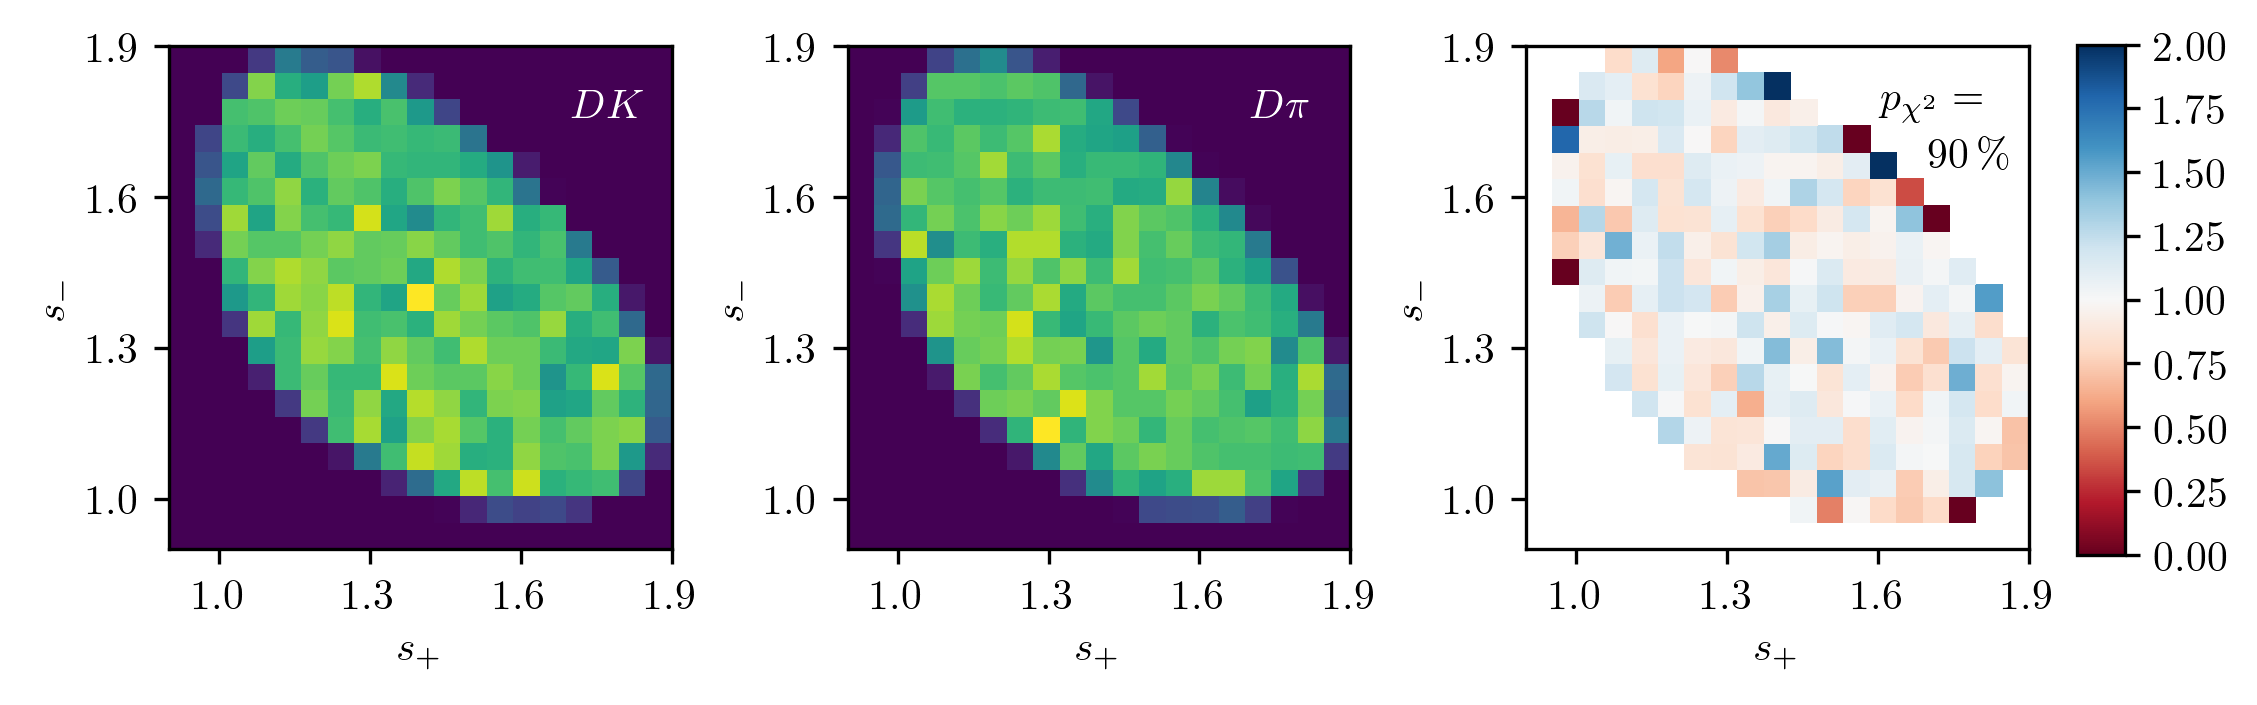
\includegraphics[width=\columnwidth]{figures/analysis/DP_thesis_m2_chi2_KK_LL.png}
    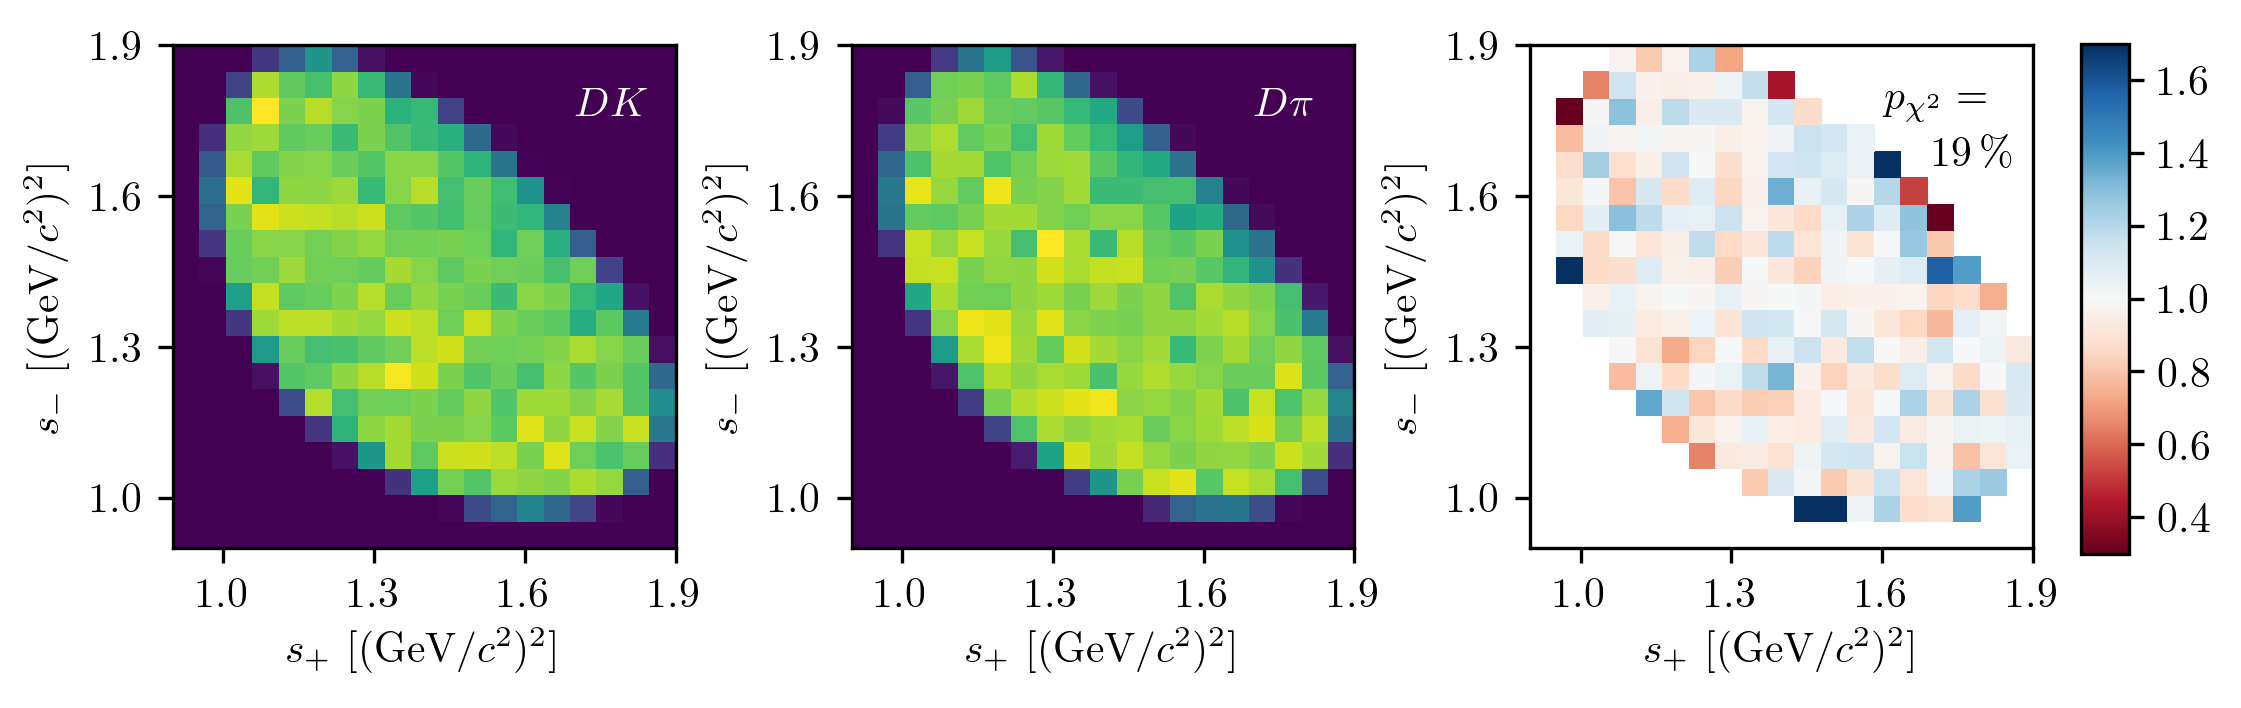
\includegraphics[width=\columnwidth]{figures/analysis/DP_thesis_m2_chi2_KK_DD.png}
    \caption{The $(s_+, s_-)$ distribution in simulated samples of (left)  $\B\to\D\kaon$ decays and (center)  $\B\to\D\pi$ decays where \DtoKsKK, as well as (right) the ratio between the two histograms (corrected for differences in sample sizes). The plots are shown for for candidates in the (top) LL and (bottom) DD categories. The $p$ values are the results of $\chi^2$ compatibility tests between the two histograms.}
    \label{fig:dk_vs_dpi_chi2_kk}
\end{figure}

This is investigated with two statistical tests. The first is a $\chi^2$ comparison of 2D histograms of the distribution of $m^2(\KS h^+)$ and $m^2(\KS h^-)$ in the different $\B\to\D\pi$ and $\B\to\D\kaon$ channels. These histograms, and the ratio between them, are shown in Figs.~\ref{fig:dk_vs_dpi_chi2_pipi}~and~\ref{fig:dk_vs_dpi_chi2_kk}, along with the $p$-values from the $\chi^2$ tests. It can be seen that, in all cases, the probability of obtaining the two histograms assuming that they share the same underlying distribution has a reasonable value, and that there is no clear trend in the ratio plots. The second test is a Kolmogorov-Smirnov test~\cite{kolmogorovSullaDeterminazioneEmpirica1933,*smirnovTableEstimatingGoodness1948} of the compatibility of the one-dimensional distributions of $m^2(\KS h^+)$, $m^2(\KS h^-)$, and $m^2(h^+ h^-)$. These distributions, and the corresponding $p$-values, are shown in Fig.~\ref{fig:KolSmi_PiPi}~and~\ref{fig:KolSmi_KK}. Again, all the $p$ values are reasonable. Therefore, it is concluded that there are no statistically significant differences between the phase-space dependence of the reconstruction and selection efficiency between the $\B\to\D\pi$ and $\B\to\D\kaon$ channels, given the present sample sizes. Because the simulation samples have approximately the same amount of decays as data (or significantly more, in the $\B\to\D\kaon$ case), any potential differences will be negligible with data yields. Thus, sharing the \Fi parameters between the $\B\to\D\pi$ and $\B\to\D\kaon$ channels is viable, and no efficiency correction is necessary. 

\begin{figure}[tbp]
    \centering
    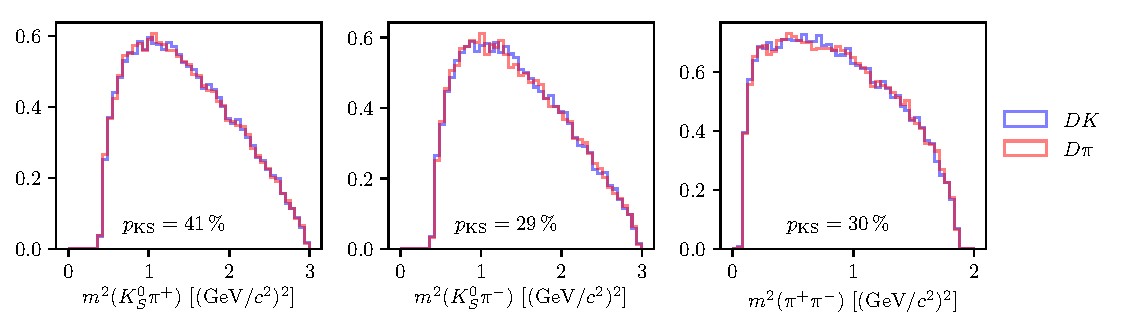
\includegraphics[width=\columnwidth]{figures/analysis/DP_thesis_s_KolSmi_PiPi_LL.pdf}
    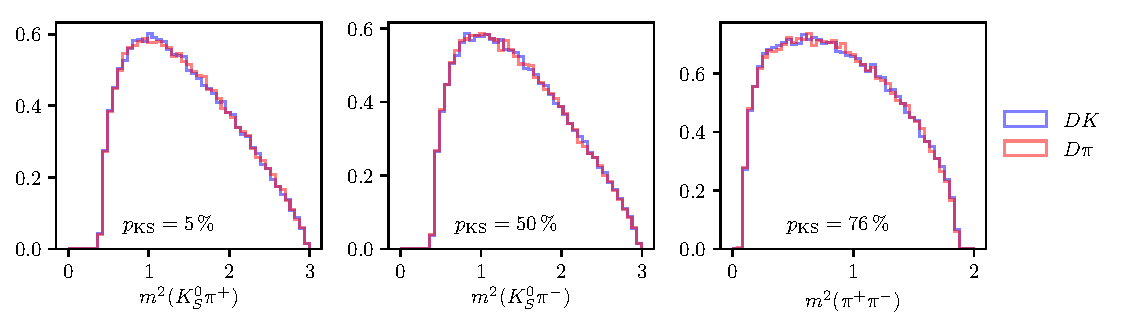
\includegraphics[width=\columnwidth]{figures/analysis/DP_thesis_s_KolSmi_PiPi_DD.pdf}
    \caption{One-dimensional distributions of $m^2(\KS\pip)$, $m^2(\KS\pim)$, and $m^2(\pip\pim)$ in simulated (blue) \BtoDK and (red) \BtoDpi  decays where \DtoKspipi in the (top) LL and (bottom) DD categories. The $p$ values are the results of Kolmogorov-Smirnov compatibility tests between the distributions.}
    \label{fig:KolSmi_PiPi}
\end{figure}

\begin{figure}[tbp]
    \centering
    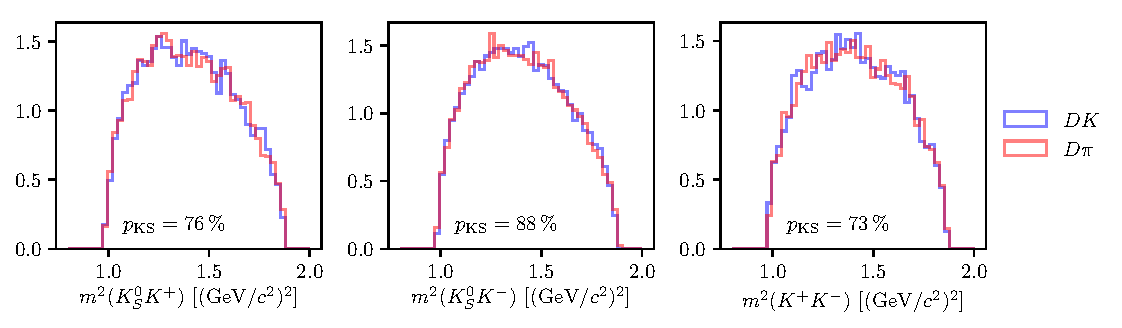
\includegraphics[width=\columnwidth]{figures/analysis/DP_thesis_s_KolSmi_KK_LL.pdf}
    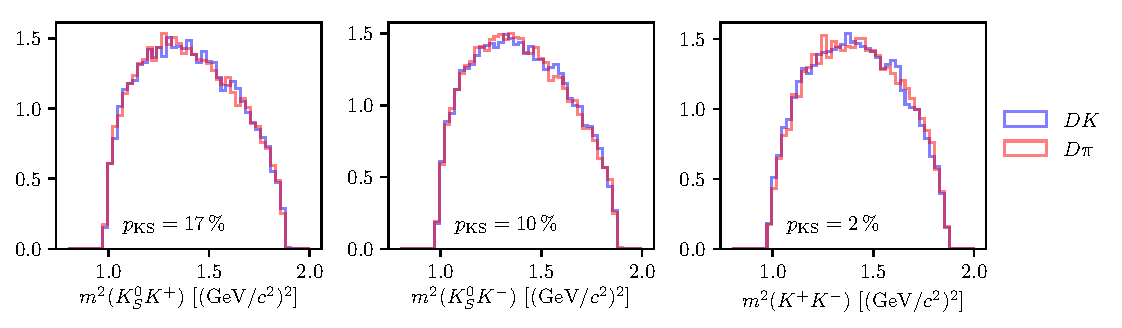
\includegraphics[width=\columnwidth]{figures/analysis/DP_thesis_s_KolSmi_KK_DD.pdf}
    \caption{One-dimensional distributions of $m^2(\KS\Kp)$, $m^2(\KS\Km)$, and $m^2(\pip\pim)$ in simulated (blue) \BtoDK and (red) \BtoDpi  decays where \DtoKsKK  in the (top) LL and (bottom) DD categories. The $p$ values are the results of Kolmogorov-Smirnov compatibility tests between the distributions.}
    \label{fig:KolSmi_KK}
\end{figure}
% subsection efficiency_profile_over_the_dalitz_plot (end)

% section signal_selection_efficiencies (end)


\section{Background studies} % (fold)
\label{sec:background_studies}

A wide range of backgrounds can potentially pollute the sample of signal candidates. The backgrounds group into three categories depending on how they are treated in the analysis: 
\begin{itemize}
    \item Backgrounds that can be effectively removed in the selection
    \item Backgrounds that are only present at a level where the impact on the measurement result is small, and which do therefore not have to be modelled
    \item Backgrounds that are present at a level where they have to be modelled in the fit to data, and cannot effectively be rejected further in the selection
\end{itemize}
The latter category comprises of combinatorial background, which remains present at a non-negligible level after the application of the BDT described in Section~\ref{sub:boosted_decision_tree};  contributions from a number of partly reconstructed $\B\to\D h^\pm X$ decays, where $X$ denotes a pion or photon that is not included in the reconstructed decay, and which can only be separated from signal decays by their $m(Dh)$ distribution; and finally \BtoDpi decays that are categorised as \BtoDK decays in the particle-identification step and vice-versa. These background sources are described in detail in Section~\ref{sec:signal_and_background_components}. This section focuses on backgrounds that led to specific requirements in the selection or proved to be small enough to not merit special treatment.

\subsection{Charmless decays} % (fold)
\label{sub:charmless_decays}


% subsection charmless_decays (end)


There is potentially a so-called \emph{charmless} background present in data, consisting of $\Bpm\to\KS h^+ h^- {h'}^\pm$ decays. These have the same final state as the signal decay, but no intermediate \D meson. Because all final state particles are reconstructed, this background peaks in the \B mass spectrum.
This background is suppressed by requiring the reconstructed \B and \D decay vertices to be separated in the $z$ direction; specifically by requiring that $\Delta z^{D-B}_{\text{significance}} > 0.5$, where $\Delta z^{D-B}_{\text{significance}}$ was defined in Eq.~\eqref{eg:Dz_sig_def}. The remaining background level can be investigated by investigating the \D mass sidebands. 

However, the use of the \texttt{DecayTreeFitter} $\chi^2_\mathrm{DTF}$ as an input variable in the BDT \emph{removes} essentially all of the \D (and \KS) sideband, due to the mass constraints in the decay chain fit. Therefore separate BDT's are trained for LL and DD candidates without the $\chi^2_\mathrm{DTF}$ as an input variable, and used when selecting candidates for the background studies presented in this section, and the following. In a similar manner, all mass window requirements are made on the \emph{default} reconstructed masses, obtained with no use of \texttt{DecayTreeFitter}. The overlap of the two sets of selected candidates in the signal \B-mass window is above 95\,\%.

\begin{figure}[tbp]
    \centering
    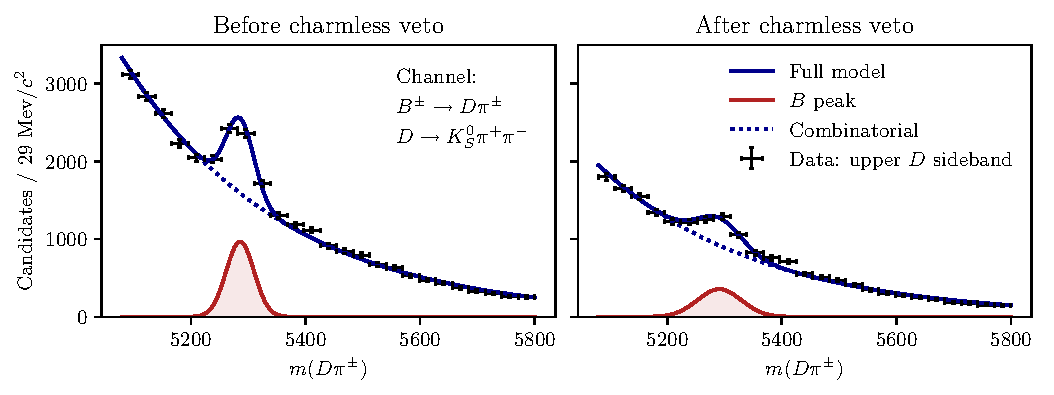
\includegraphics[width=0.95\columnwidth]{figures/analysis/background_checks/charmless_Pi_PiPi.pdf}
    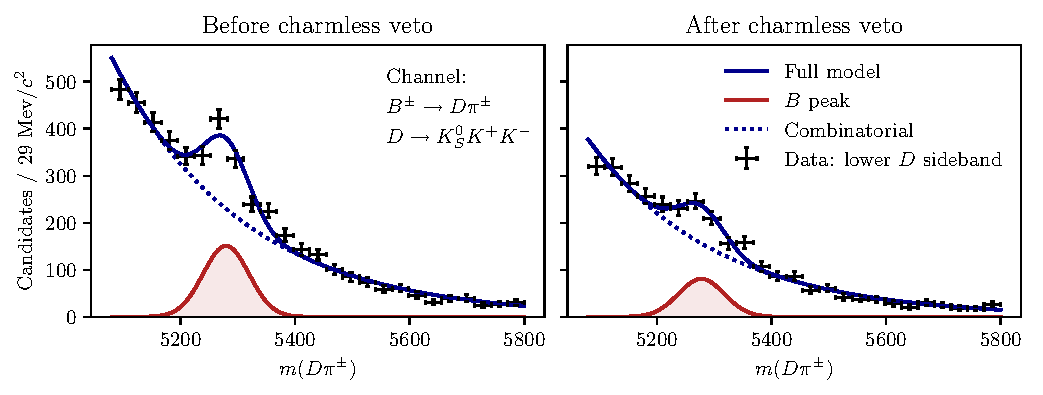
\includegraphics[width=0.95\columnwidth]{figures/analysis/background_checks/charmless_Pi_KK.pdf}
    \caption{The \B mass distribution of (top) $\Bpm\to\D(\to\KS\pip\pim)\pipm$ and (bottom) $\Bpm\to\D(\to\KS\Kp\Km)\pipm$ candidates reconstructed in both the LL and DD categories, residing in the upper \D mass sideband $m_D\in [1910, 1960]\mevcc$ for $D\to\Ks\pip\pim$ and in the lower sideband $m_D\in [1910, 1960]\mevcc$ for $\D\to\KS\Kp\Km$, with (left) no requirement on $\Delta z^{BD}_{\text{significance}}$ and (right) after a requirement of $\Delta z^{BD}_{\text{significance}} > 0.5$. }
    \label{fig:charmless_Bmass_DPi}
\end{figure}

\begin{figure}[tbp]
    \centering
    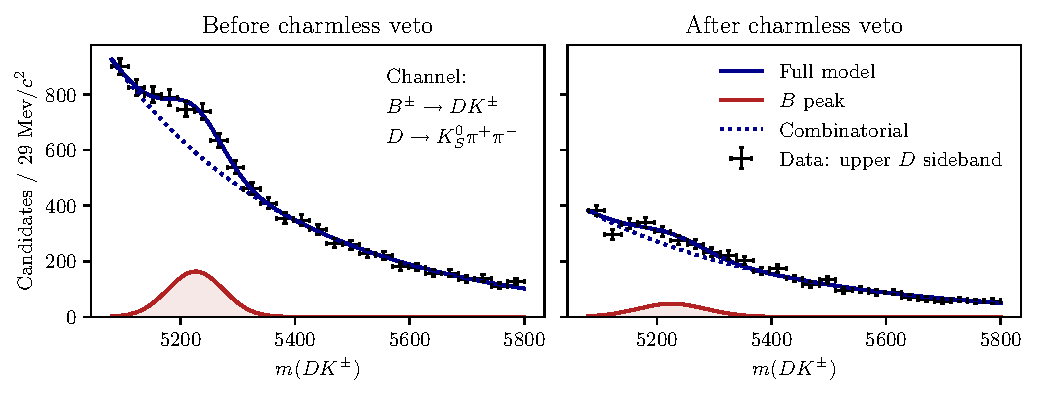
\includegraphics[width=0.95\columnwidth]{figures/analysis/background_checks/charmless_K_PiPi.pdf}
    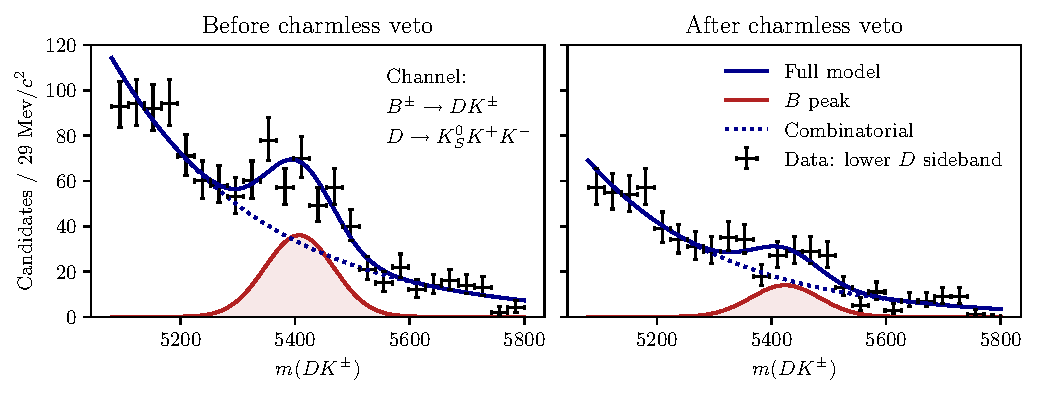
\includegraphics[width=0.95\columnwidth]{figures/analysis/background_checks/charmless_K_KK.pdf}
    \caption{The \B mass distribution of (top) $\Bpm\to\D(\to\KS\pip\pim)\Kpm$ and (bottom) $\Bpm\to\D(\to\KS\Kp\Km)\Kpm$ candidates reconstructed in both the LL and DD categories, residing in the upper \D mass sideband $m_D\in [1910, 1960]\mevcc$ for $D\to\Ks\pip\pim$ and in the lower sideband $m_D\in [1910, 1960]\mevcc$ for $\D\to\KS\Kp\Km$, with (left) no requirement on $\Delta z^{BD}_{\text{significance}}$ and (right) after a requirement of $\Delta z^{BD}_{\text{significance}} > 0.5$. }
    \label{fig:charmless_Bmass_DK}
\end{figure}



The reconstructed \B mass spectrum is shown for \BtoDpi candidates in the \D sidebands in Fig.~\ref{fig:charmless_Bmass_DPi}, both before and after making a requirement on $\Delta z^{D-B}_{\text{significance}}$. The check is based on the upper \D sideband for \DtoKspipi decays and the lower \D sideband for \DtoKsKK decays to avoid contamination from real \BtoDh decays with subsequent $\D\to\KS\Kpm\pimp$ decays, or crossfeed between the two signal \D-decay modes. A peak is clearly visible, the size of which is reduced by the requirement. This peak is partly due to a contribution from $\Bpm\to\KS\pip\pim\pipm$ decays (${\Bpm\to\KS\Kp\Km\pipm}$ decays) in the \DtoKspipi (\DtoKsKK) channel, and partly due to real signal decays that leak into the \D sidebands. The number of real signal decays can be calculated from the yield obtained in the fit of Section~\ref{sec:signal_and_background_components}, and the reconstructed $m_D$ distribution in simulated signal decays. Subtracting this contribution, it is estimated that approximately 450 (200) charmless decays are present in the \Kspipi (\KsKK) data samples. In similar fashion, Fig.~\ref{fig:charmless_Bmass_DK} shows the $m_B$ spectra for \BtoDK candidates in the \D sidebands. In these plots, the peaks are at $m_B$ values that are lower (higher) than the \B mass in the \KsPiPi (\KsKK) categories, because they stem from real $\Bpm\to\KS\Kp\Km\pipm$ decays where a kaon is mis-reconstructed as a pion or a pion is misreconstructed as a kaon, respectively. The total contribution of charmless decays in the \BtoDK data samples is estimated to be about 200 decays. As described further in Section~\ref{sub:systematics_from_charmless_backgrounds}, the presence of a charmless background at these levels has a negligible impact on the measurement results. It is not favourable to tighten the requirement further due to the associated loss in the selection efficiency of signal decays.


\subsection{\texorpdfstring{Background from four-body \D decays}{Background from four-body D decays}}% (fold)
\label{sub:background_from_four_body_d_decays}

\begin{figure}[tbp]
    \centering
    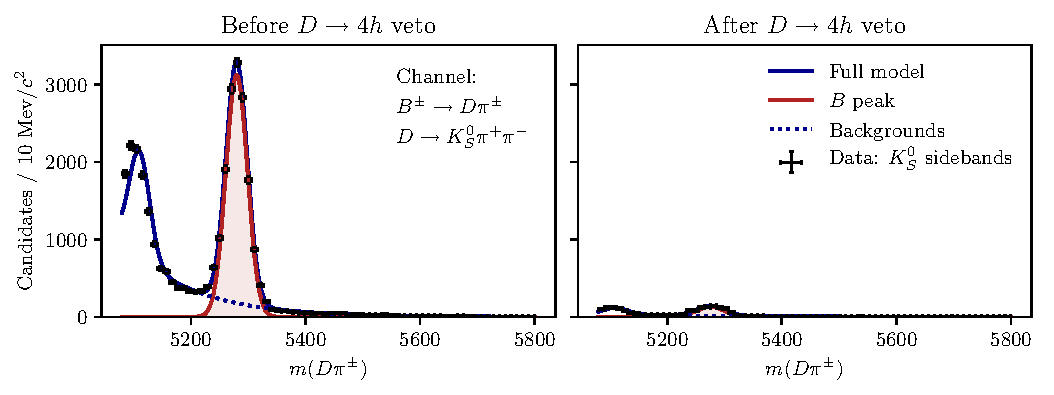
\includegraphics[width=0.95\columnwidth]{figures/analysis/background_checks/ks_fd_check_Pi_PiPi.pdf}
    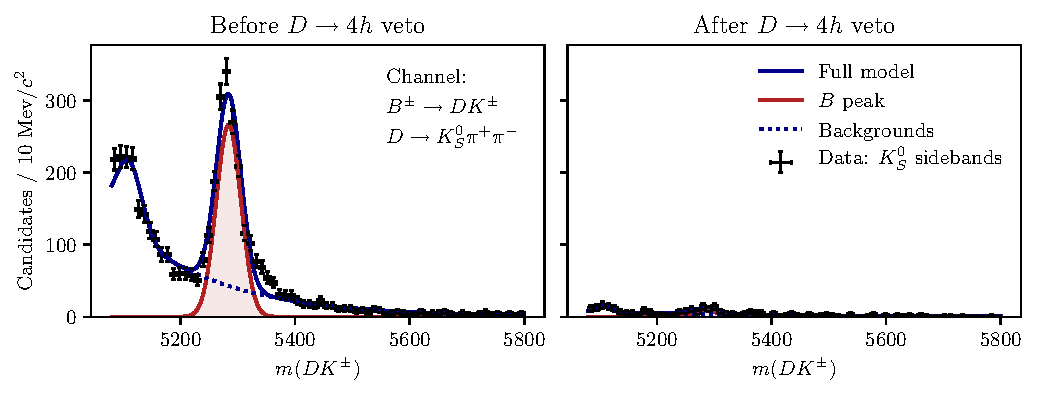
\includegraphics[width=0.95\columnwidth]{figures/analysis/background_checks/ks_fd_check_K_PiPi.pdf}
    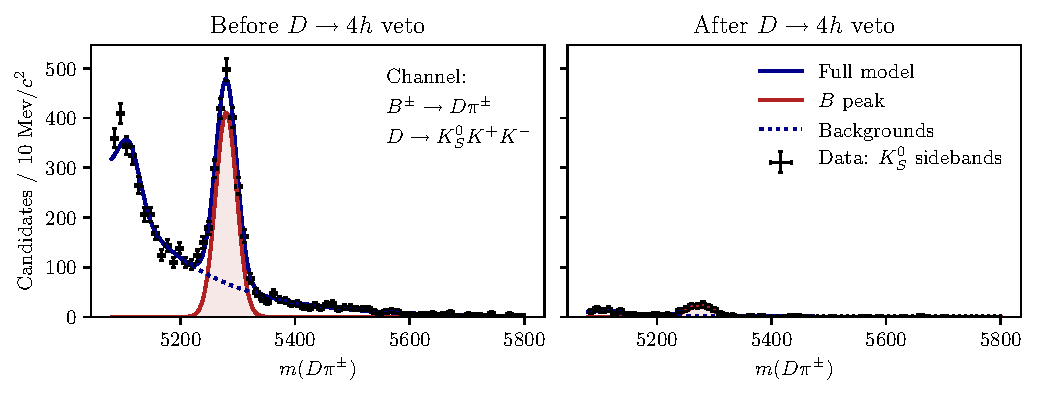
\includegraphics[width=0.95\columnwidth]{figures/analysis/background_checks/ks_fd_check_Pi_KK.pdf}
    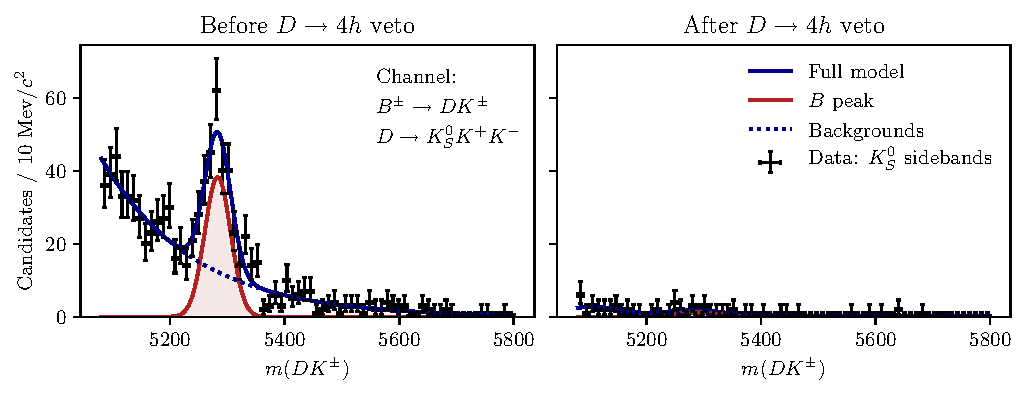
\includegraphics[width=0.95\columnwidth]{figures/analysis/background_checks/ks_fd_check_K_KK.pdf}
    \caption{The \B mass spectrum in the \KS sideband where $m_\KS\in[467, 482]\mevcc$ or $\m_\KS\in[512,527]\mevcc$ (left) without a requirement on the \KS flight distance significance, and (right) after the requirement implemented in the analysis.}
    \label{fig:fake_ks}
\end{figure}

A similar potential background is from real \BtoDh decays where the \D meson decays directly to the $\pip\pim h^+ h^-$ final state, without an intermediate \KS meson. This background can be investigated by looking for a peak in the \B mass spectrum for candidates in the \KS sideband, as illustrated in Fig.~\ref{fig:fake_ks}. The figure shows the spectrum in the final data sample, illustrating the significant effect of making the requirement on the \KS flight distance that was discussed in Section~\ref{sub:initial_requirements}. The BDT that does \emph{not} rely on the DTF $\chi^2$ has been used to suppress combinatorial background. The remaining peak after requiring $\chi^2_\text{FD}>49$ is completely accounted for by real signal decays that leak into the \KS sideband. The requirement is made for candidates in the LL category only; if the pions stemming from a \KS candidate are reconstructed as downstream tracks it implies that the \KS has travelled from the interaction region.

% subsection texorpdfstring_background_from_four_body_d_decays (end)

\subsection{Semi-leptonic backgrounds} % (fold)
\label{sub:semi_leptonic_backgrounds}



The data sample has a minor background from $\B\to\D\mu\nu_\mu X$ decays, visible in the \B mass spectrum when the companion is required to satisfy $\texttt{isMuon=1}$.  This is shown in Fig.~\ref{fig:semileptonic_B_check_mu} for both the \BtoDK and \BtoDpi channels where \DtoKspipi. The \B mass spectra for simulated $\Bpm\to\D\mupm\nu_\mu$ decays reconstructed in each category are also shown, from simulation samples produced via \texttt{RapidSim}. The background is very efficiently vetoed by requiring $\texttt{IsMuon=0}$ on the companion. This requirement removes approximately 85\,\% of the background decays, as estimated using the \texttt{PIDCalib} calibration samples and the $(p, p_T)$ distribution for the muon in the \texttt{RapidSim} samples. The fraction of signal candidates for which the companion satisfies $\texttt{IsMuon=1}$ in simulated signal samples is $\leq 0.9\,\%$ so the impact on signal yield is small.

\begin{figure}[tb]
    \centering
    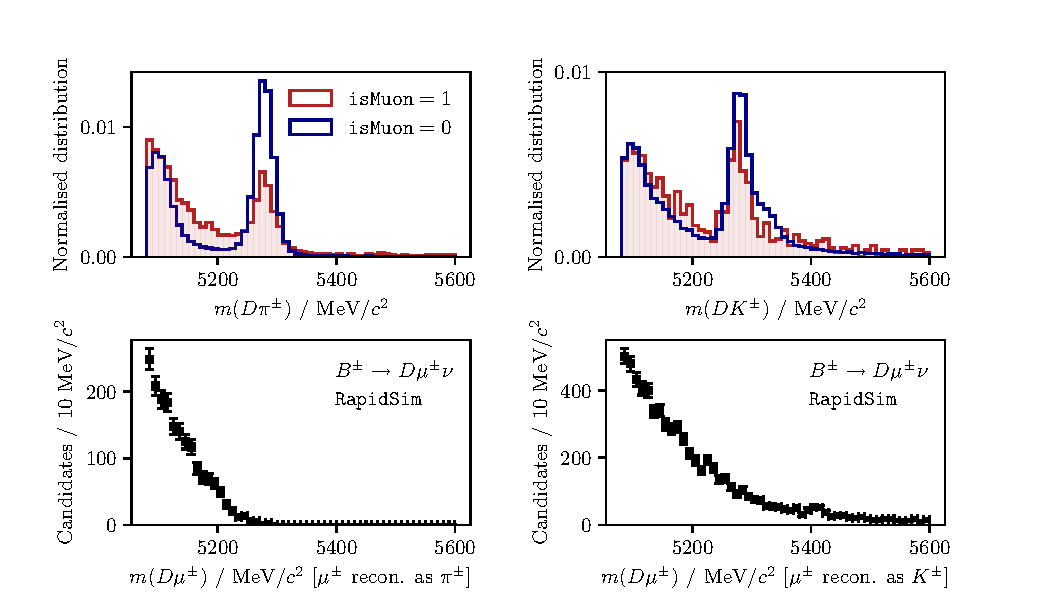
\includegraphics[width=\columnwidth]{figures/analysis/background_checks/b2dmunu_plot.pdf}
    \caption{(Top) The $m_B$ spectra in data split by the value of $\texttt{isMuon}$ for the companion particle, in (left) the $\Dpi$ and (right) the $\DK$ samples where \DtoKspipi. The two histograms are normalised independently, so that the distributions can be compared. The fractions of candidates in data (with $m_B\in[5080, 5800]\mevcc$) where the companion satisfies $\texttt{isMuon=1}$ are 1.6\,\% and 1.8\,\% for the $\Dpi$ and $\DK$ channels respectively. (Bottom) the \texttt{RapidSim} mass spectra for $\Bpm\to\Dz\mupm\nu_\mu$ decays reconstructed in the (left) $\Dpi $and (right) $\DK$ categories.}
    \label{fig:semileptonic_B_check_mu}
\end{figure}

The analogous $\B\to\D e\nu_e X$ background is investigated by inspecting the \B mass spectra after making requirements on \texttt{PIDe} for the companion candidate, but a presence of the semi-leptonic background in data is not visible and no electron veto is applied to the companion.


\subsubsection{Background from semi-leptonic D decays} % (fold)
\label{ssub:background_from_semi_leptonic_d_decays}

\begin{figure}[tbp]
    \centering
    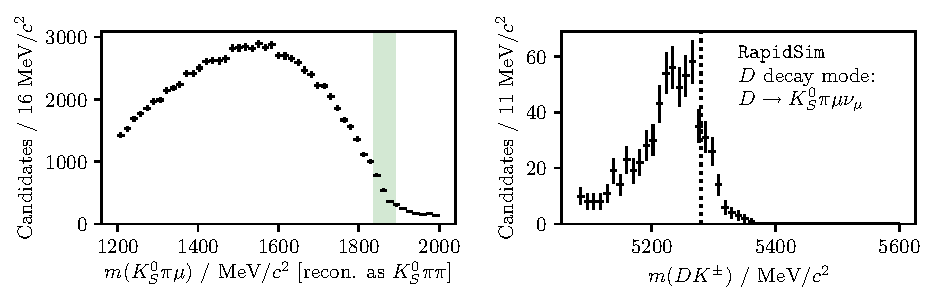
\includegraphics[width=0.8\columnwidth]{figures/analysis/background_checks/semilep_D_mu_PHSP.pdf}
    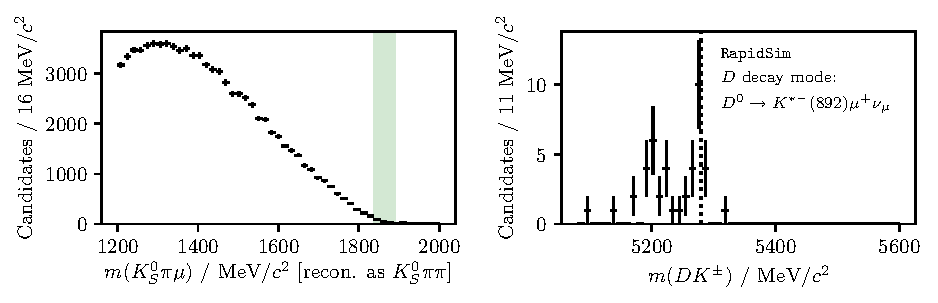
\includegraphics[width=0.8\columnwidth]{figures/analysis/background_checks/semilep_D_mu_892.pdf}
    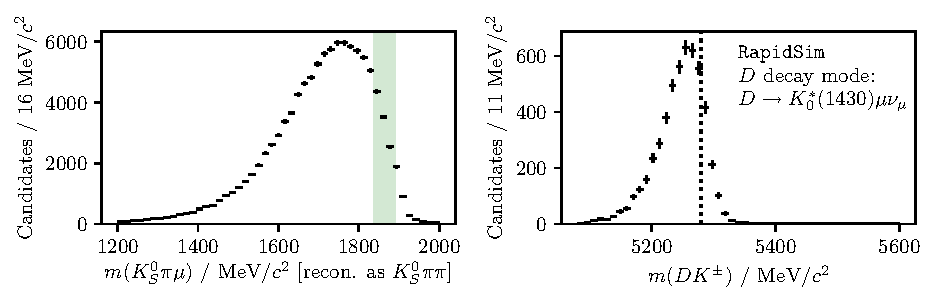
\includegraphics[width=0.8\columnwidth]{figures/analysis/background_checks/semilep_D_mu_1430.pdf}
    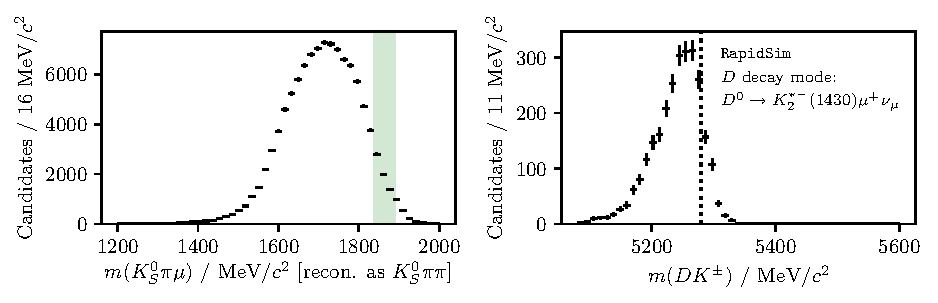
\includegraphics[width=0.8\columnwidth]{figures/analysis/background_checks/semilep_D_mu_1430_2.pdf}
    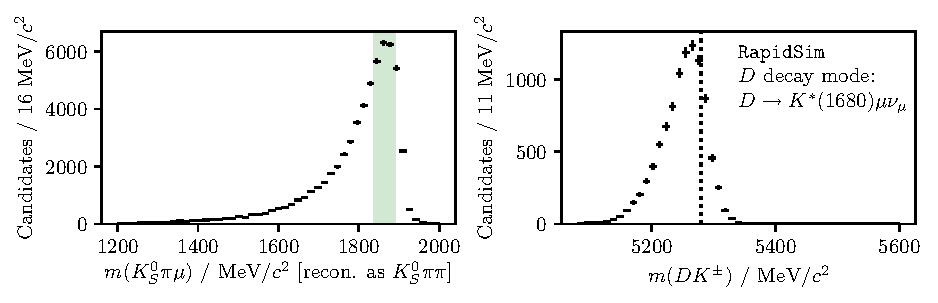
\includegraphics[width=0.8\columnwidth]{figures/analysis/background_checks/semilep_D_mu_1680.pdf}
    \caption{The reconstructed (left) $m(\KS \pi^+ \pi^-)$ and (right) $m(Dh)$ distributions in \texttt{RapidSim} samples of $\Bpm\to\D \Kpm$ decays where $\Dz\to\KS\pi^-\mu^+\nu_\mu$. The top plot is for  decays the were uniformly distributed over phase space, and the following plots show the distribution where the $\KS\pim$ originate in the resonances $\Kstarm(892)$, $K^{*-}_0(1430)$, $K^{*-}_2(1430)$, and $\Kstarm(1680)$. The shapes for the $\Dz\to\KS\pi^-e^+\nu_e$ case are almost identical.}
    \label{fig:semileptonic_D_decays_kspp}
\end{figure}

\begin{figure}[tp]
    \centering
    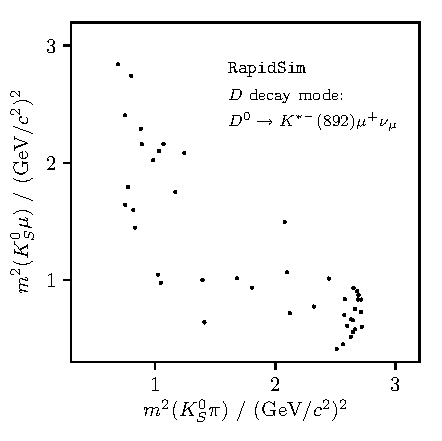
\includegraphics[width=0.35\columnwidth]{figures/analysis/background_checks/semilep_d_DP_892.pdf}
    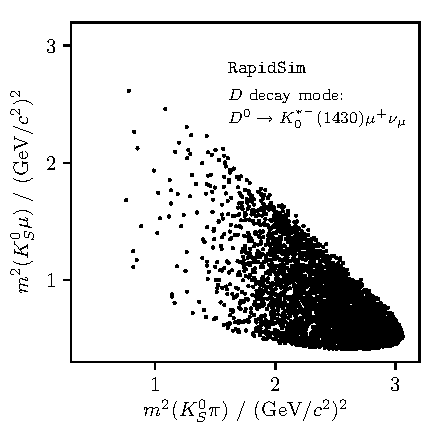
\includegraphics[width=0.35\columnwidth]{figures/analysis/background_checks/semilep_d_DP_1430.pdf}
    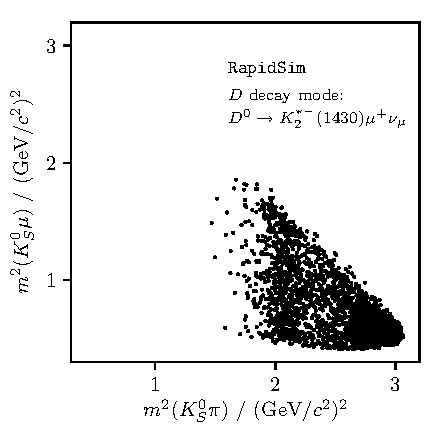
\includegraphics[width=0.35\columnwidth]{figures/analysis/background_checks/semilep_d_DP_1430_2.pdf}
    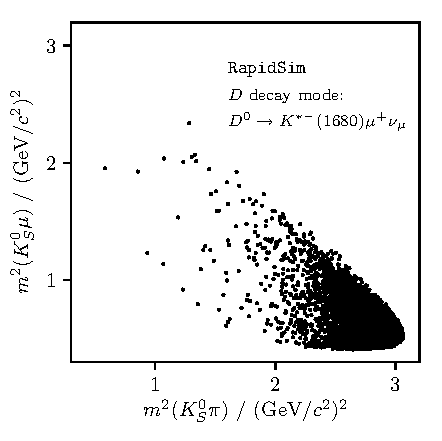
\includegraphics[width=0.35\columnwidth]{figures/analysis/background_checks/semilep_d_DP_1680.pdf}
    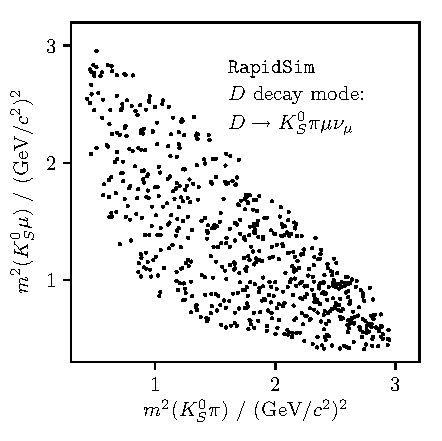
\includegraphics[width=0.35\columnwidth]{figures/analysis/background_checks/semilep_d_DP_PHSP.pdf}
    \caption{Dalitz distribution for $\D\to\KS\pi\mu\nu_\mu$ decays in \texttt{RapidSim}, where the $\KS\pim$ originate in the resonances $\Kstarm(892)$, $\Kstarm_0(1430)$, $\Kstarm_2(1430)$, and $\Kstarm(1680)$, as well as for a uniform distribution over phase space.}
    \label{fig:d2kstmunu_dalits}
\end{figure}

There is a potential background from real $\Bpm\to\D h^\pm$ decays where the \D meson decays semi-leptonically: $\Dz\to\KS\pim\ell^+\nu_\ell$. This background is particularly dangerous because is peaks at the \B mass, when the \D-mass requirement is applied and it is reconstructed in the \DtoKspipi category. This is illustrated in Fig.~\ref{fig:semileptonic_D_decays_kspp} using \texttt{RapidSim} samples of $\Bpm\to\D(\to K^{*-}(\to \KS\pi-)\ell^+\nu_\ell)h^\pm $ decays for $K^{*}\in=\{K^*(892), K^*_0(1430), K^*_2(1430), K^*(1680)\}$. The respective spin of each resonance is taken into account in generation, by handling the decay via \evtgen. The expected background yields relative to signal can be estimated by applying the \B and \D mass cuts to decays in the \texttt{RapidSim} samples, and using the relative branching ratios. Only the $\Dz\to\Kstarm(892)\ell\nu_\ell$ branching fractions have been measured~\cite{PDG2020}, but there is no reason to expect that higher \Kstar resonances should not contribute. To estimate their potential contribution, the branching ratios are approximated by
\begin{align*}
    \text{BR}&[\Dz\to\Kstarm(X)(\to\KS\pim)\ell\nu_\ell] \simeq\\& \frac{\text{BR}[\Dz\to\Kstarm(X)(\to\KS\pim)\pip] }{\text{BR}[\Dz\to\Kstarm(892)(\to\KS\pim)\pip] }\text{BR}[\Dz\to\Kstarm(892)(\to\KS\pim)\ell\nu_\ell] 
\end{align*}
because all the relevant $\Dz\to\Kstarm(\to\KS\pim)\pip$ branching fractions are known~\cite{PDG2020
}. The efficiencies and branching ratios relative to the signal channel are given in Table~\ref{tab:relative_d2ksellnu_yields}. It is clear that the higher \Kstar resonances are important: the smaller branching ratios are compensated for by a higher selection efficiency, due to the smaller phase-space of the missed neutrino. The total background yield is 1.1\,\% of the signal yield in both the \BtoDpi and \BtoDK channels. However, there will be an additional contribution in the \BtoDK channel from real \BtoDpi decays with semi-leptonic \D decays and a mis-identification of the companion. This background also peaks, and the yield is approximately 0.4\,\% of the \BtoDK signal yield.

\begin{table}
    \centering
    \caption{The selection efficiencies of $\Bpm\to\D\Kpm$ decays where $\Dz\to\KS\pim\ell^+\nu_\ell$ when reconstructed in the \DtoKspipi mode in \texttt{RapidSim} relative to the signal selection efficiencies, for a number of decay modes: $\texttt{PHSP}$ as well as resonant production where the $\KS\pim$ pair originates in one of several \Kstar resonances. The relative branching ratios are also shown, calculated as explained in the main text, as well as the predicted relative yields.
    \label{tab:relative_d2ksellnu_yields}}
    \begin{tabular}{l |cc|c}
    \toprule
    Mode & $\epsilon_{bkg}/\epsilon_{signal}$ (\%)& $\Gamma_{bkg}/\Gamma_{signal}$ (\%)& $N_{bkg}/N_{signal}$ (\%)\\
    \midrule

    $\D\to\KS\pim\mu^+\nu_{\mu}$ (\texttt{PHSP})     & $0.92 \pm 0.05$ & $18.3 \pm 14.8$ & $0.17 \pm 0.14$\\
    $\D\to (\KS\pim)_{K^{*-}(892)}\mu^+\nu_{\mu}$    & $0.06\pm0.01$ & $22.3\pm 3.2$ & $0.013 \pm 0.003$ \\
    $\D\to (\KS\pim)_{K^{*-}_0(1430)}\mu^+\nu_{\mu}$ & $7.3 \pm 0.1$ & $3.7 \pm 0.8$ & $0.27 \pm 0.06   $\\
    $\D\to (\KS\pim)_{K^{*-}_2(1430)}\mu^+\nu_{\mu}$ & $3.7 \pm 0.1$ & $0.5 \pm 0.3$ & $0.02 \pm 0.01$   \\
    $\D\to (\KS\pim)_{K^{*-}(1680)}\mu^+\nu_{\mu}$   & $24.4 \pm 0.3$ & $0.6 \pm 0.5$ & $0.15 \pm 0.12$\\
    \midrule
    $\D\to\KS\pim e^+\nu_{e}$ (\texttt{PHSP})       & $0.53\pm0.02$ & $20.8\pm16.3$ & $0.11 \pm 0.09$\\
    $\D\to (\KS\pim)_{K^{*-}(892)} e^+\nu_{e}$      & $0.15\pm0.02$ & $25.6 \pm 2.5$ & $0.04 \pm 0.01$\\
    $\D\to (\KS\pim)_{K^{*-}_0(1430)} e^+\nu_{e}$   & $6.3 \pm 0.1$ & $4.2\pm0.8$ & $0.26\pm0.05$\\
    $\D\to (\KS\pim)_{K^{*-}_2(1430)} e^+\nu_{e}$   & $4.12 \pm 0.08$ & $0.5 \pm 0.3$ & $0.02\pm0.01$\\
    $\D\to (\KS\pim)_{K^{*-}(1680)} e^+\nu_{e}$     & $10.0 \pm 0.2$ & $0.7 \pm 0.5$ & $0.07\pm0.05$\\
    \midrule
    Total & - & - & $1.1\pm0.4$\\
    \bottomrule
    \end{tabular}
\end{table}

% \begin{figure}[tbp]
%     \centering
%     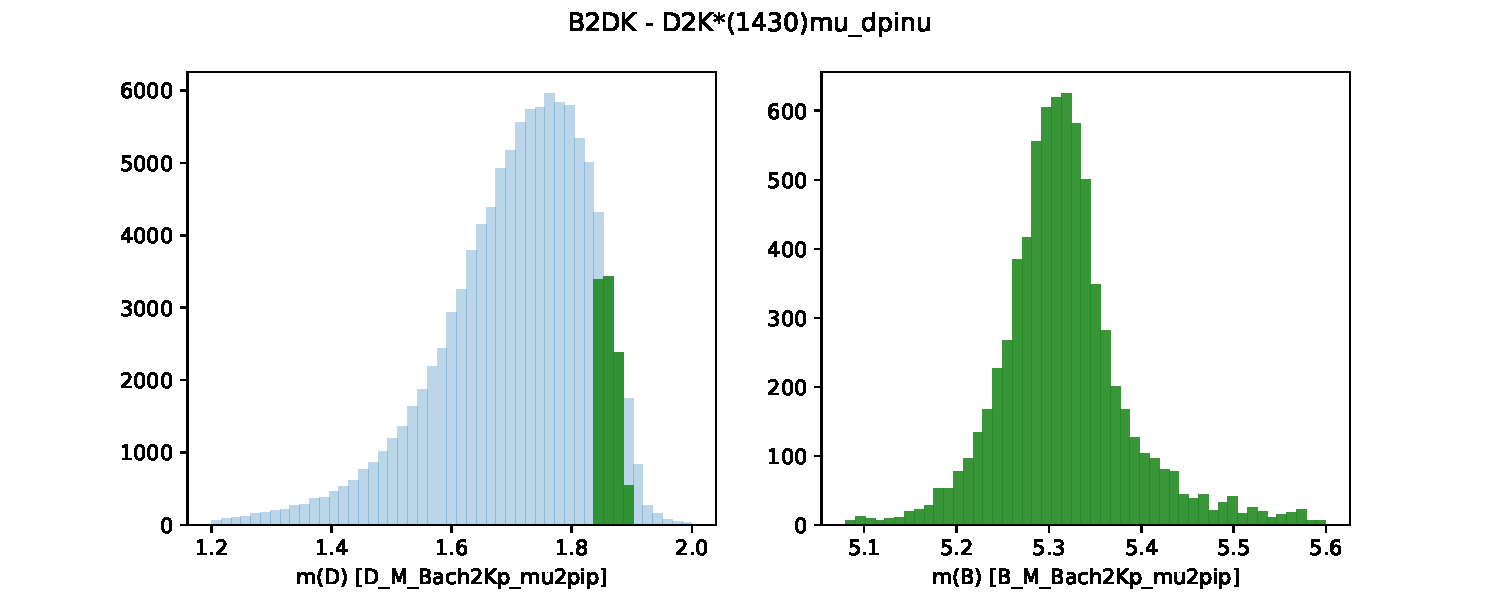
\includegraphics[width=0.9\columnwidth]{figures/analysis/semileptonic_bkgs/D2Kspimunu_with_misID.pdf}
%     \caption{The reconstructed (left) $m(\KS \pi^+ \pi^-)$ and (right) $m(Dh)$ distributions in RapidSim samples of $\Bpm\to\D \pipm$ decays where $\Dz\to K^{*-}_0(1430)(\to \KS\pi^-)\mu^+\nu_\mu$, where the bachelor pion is misidentified as a kaon.}
%     \label{fig:semileptonic_D_decays_kspp_misID}
% \end{figure}

\begin{figure}[tb]
    \centering
    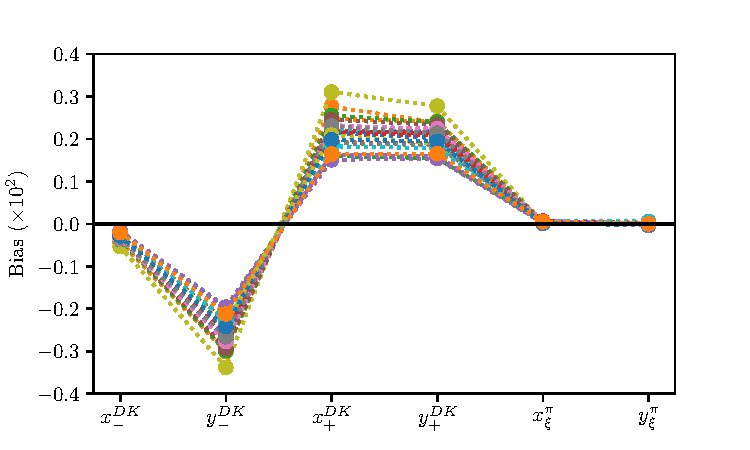
\includegraphics[width=0.65\columnwidth]{figures/analysis/background_checks/D2Kstmunu_biases.pdf}
    \caption{Estimated biases on the measured observables due to the presence of $\D\to\KS\pi\ell\nu_\ell$ backgrounds, calculated while varying efficiencies and branching ratios within uncertainties.}
    \label{fig:d2kstmunu_biases}
\end{figure}

The potential impact from the presence of the background is estimated by 
\begin{enumerate}
    \item calculating the expected \BtoDpi and \BtoDK signal yields in each bin for physics parameters similar to the world average values
    \item then calculating the background bin yields in each bin, using the relative branching fractions and efficiencies described above and taking the bin-distribution from the \texttt{RapidSim} samples. The \texttt{RapidSim} samples are produced using the \texttt{ISGW2} model in \evtgen~\cite{EvtGen}, yielding the Dalitz distributions in Fig.~\ref{fig:d2kstmunu_dalits}.
    \item adding the signal and background yields, and fitting the new \BtoDpi and \BtoDK yields back with the default signal-yield expressions (including a fit of the \Fi parameters)
\end{enumerate}
The obtained biases are shown in Fig.~\ref{fig:d2kstmunu_biases}, where they are calculated a number of times, each time varying the efficiencies within statistical uncertainties and the relevant branching fractions within the measurement uncertainties. The  systematic uncertainty due to the unknown branching fractions and the use of \texttt{RapidSim} in lieu of full simulation is not included, but is of course significant. Nevertheless it is clear that the potential biases are significant compared to the size of the systematic uncertainties of the analysis presented in Section~\ref{sec:systematic_uncertainties}. Therefore the backgrounds are vetoed by requiring $\texttt{IsMuon=0}$ and $\texttt{PIDe} < 0$ on the pions from the \D-decay with opposite charge to the bachelor in the \DtoKspipi channel. This requirement removes 88\,\% of the muonic background and 99\,\% of the electron background, according to PID efficiencies obtained via the  \texttt{PIDCalib} package, using the $(p, p_T)$ distribution for the muon/electron in the \texttt{RapidSim} samples. The survival rate for signal decays in full simulation is 94\,\%, so the impact on the obtainable precision is only about $3\,\%$. A systematic uncertainty is assigned to account for the potential remaining background.

\begin{figure}[tbp]
    \centering
    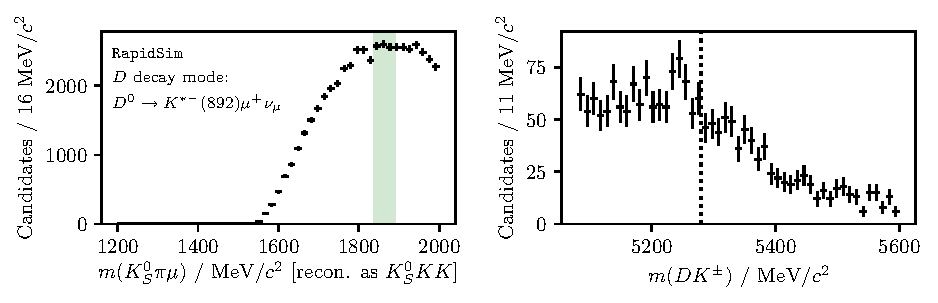
\includegraphics[width=0.8\columnwidth]{figures/analysis/background_checks/semilep_D_mu_892_KsKK.pdf}
    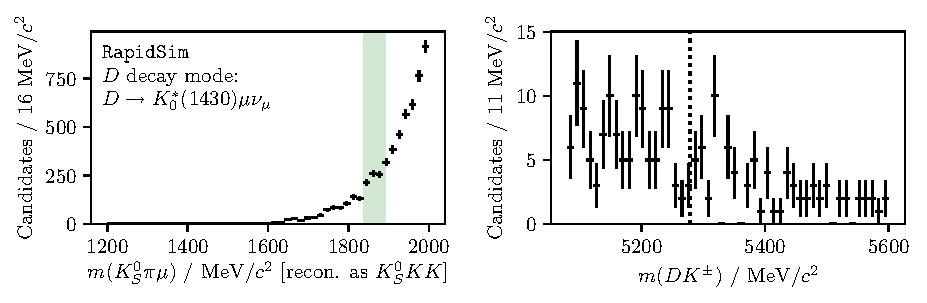
\includegraphics[width=0.8\columnwidth]{figures/analysis/background_checks/semilep_D_mu_1430_KsKK.pdf}
    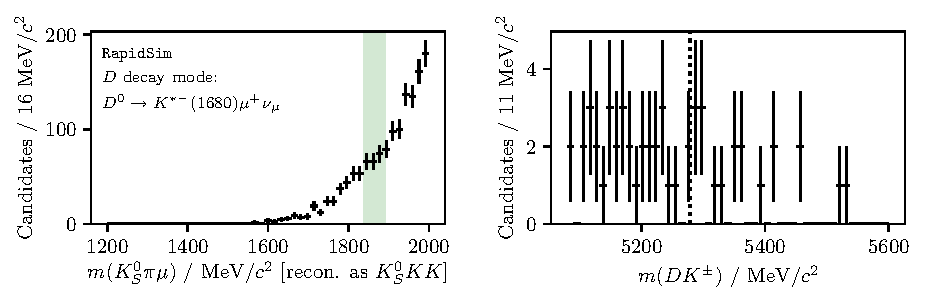
\includegraphics[width=0.8\columnwidth]{figures/analysis/background_checks/semilep_D_mu_1680_KsKK.pdf}
    \caption{The reconstructed (left) $m(\KS K^+ K^-)$ and (right) $m(Dh)$ distributions in \texttt{RapidSim} samples of $\Bpm\to\D \Kpm$ decays where $\Dz\to\KS\pi^-\mu^+\nu_\mu$, where the $\KS\pim$ originate in (top to bottom) the resonances $\Kstarm(892)$, $K^{*-}_0(1430)$, and $\Kstarm(1680)$. The shapes for the $\Dz\to\KS\pi^-e^+\nu_e$ case are almost identical.}
    \label{fig:semileptonic_D_decays_kskk}
\end{figure}

% In the final data sample 6\,\% of the \D-decay products on which the veto is applied are outside the muon acceptance, and 6\,\% are outside the ECAL acceptance. Assuming these fractions to be the same for the semileptonic backgrounds, the rejection factors may be 82\,\% and 93\,\%, respectively, instead of 88\,\% and 99\,\%. While the systematic is assigned assuming the larger rejection rates, the obtained uncertainties are negligible, and thus the acceptance effect does not pose a problem.

In the $\DtoKskk$ channel an analogous study shows the relative yields to be similar. The selection efficiencies are higher, as are the relative branching ratios due to the lower \DtoKskk branching fraction, but in this mode the $\texttt{PIDK}>-5$ requirement placed on the pion and lepton removes approximately 90\,\% of the background, leaving the relative rate similar to in \DtoKspipi. However, importantly, \emph{the background is not peaking}, as shown in Fig.~\ref{fig:semileptonic_D_decays_kskk}. The presence of a percent-level, \emph{non-peaking} background in the \DtoKskk channel is safe to ignore and thus no veto is applied to remove semileptonic \D decays in the \DtoKskk channel.

% subsubsection background_from_semi_leptonic_d_decays (end)

% Decay-flight-flight

The muon-veto for the semi-leptonic background does remove some signal decays, where an original pion or kaon results in hits in the muon detectors. A significant contribution is from particles that decay in flight. The track quality of these decays is worse than for nominal decays, which affects the resolution on the reconstructed Dalitz coordinates. In simulated signal decays the standard deviation of $\Delta m^2_\pm = m^2_{reco}(\KS\pipm)-m^2_{TRUE}(\KS\pipm)$ is 50\,\% larger for decays where one of the \D-decay products has $\texttt{IsMuon=1}$ than in decays where this is not the case. This can lead to systematic biases on the observables, as described further in Section~\ref{sub:dalitz_plot_bin_migration}. The overall effect is small, as evidenced by the systematic uncertainty described in that section; nevertheless this fact motivates removing decay-in-flight decays of the \D-decay products. Therefore it is also required that $\texttt{IsMuon=0}$ for the \D-decay pion with the same charge as the companion in the \DtoKspipi channels, and on the \D-decay kaons in the \DtoKskk channels. This veto removes about 2\,\% of signal candidates in simulation that survive the lepton vetoes described in the previous sections.


\subsection{\texorpdfstring{Cross-feed from other $\D\to\KS h^+h'^-$ decays}{Cross-feed from other D->KShh' decays}} % (fold)
\label{sub:cross_feed_from_other_d_kshh_decays}

Misidentification of a \D decay product can lead to background from cross-feed between the ${\Bpm\to\D(\to\Ks\pip\pim)h^\pm}$ and ${\Bpm\to\D(\to\Ks\Kp\Km)h^\pm}$ signal channels, or cross-feed from ${\Bpm\to\D(\to\Ks\kaon\pi)h^\pm}$ decays into either of the signal channels. However, this background is very highly suppressed by the employed requirement on the \D mass. This is illustrated in Fig.~\ref{fig:KsKpi}, where the \D mass distribution in samples of simulated $\Bpm\to\D(\to\Ks\kaon\pi)\kaon^\pm$  decays are shown, when reconstructed as $\D\to\KS\pip\pim$ and $\D\to\KS\Kp\Km$ decays. Essentially no decays that fall in the selected \D mass window survive the full selection. Therefore this background is not considered further. Neither is the background due to cross-feed between $\Bpm\to\D(\to\Ks\pip\pim)h^\pm$ and $\Bpm\to\D(\to\Ks\Kp\Km)h^\pm$, since it involves two misidentified particles, and therefore will result in reconstructed \D masses even further away from the selected mass window. A very loose PID requirement on the charged \D decay products is nonetheless included in the \DtoKsKK channel, because it helps reduce the level of combinatorial background.

\begin{figure}[tbp]
    \centering
    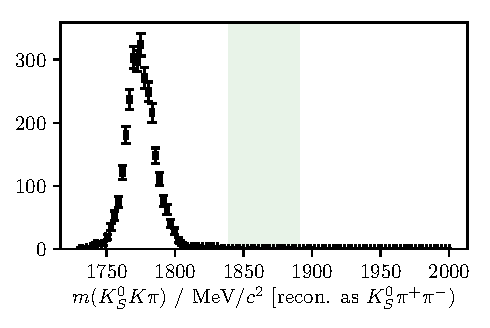
\includegraphics[width=0.45\columnwidth]{figures/analysis/background_checks/pretty_KsKpi_check_PiPi.pdf}
    \includegraphics[width=0.45\columnwidth]{figures/analysis/background_checks/pretty_KsKpi_check_KK.pdf}
    \caption{Simulated samples of $\Bpm\to\D(\to\Ks\kaon\pi)\pi^\pm$ decays reconstructed in the (left) \DtoKspipi and (right) \DtoKsKK channels, combining the LL and DD categories. The \D-mass region included in the selection of signal decays is illustrated with the green band. The plots in the \BtoDK channels look almost identical.}
    \label{fig:KsKpi}
\end{figure}




% subsection cross_feed_from_other_d_kshh_decays (end)

\subsection{Swapped-track backgrounds} % (fold)
\label{sub:swapped_track_backgrounds}

A possible peaking background stems from real $\B\to\D h X$ decays with the same final state tracks as in the signal case, but where some tracks are mis-assigned in the reconstruction. Examples are $\Bp\to(\KS h^+h'^-)_Dh^+$ decays where the companion and the \D-decay product with the same charge are swapped, or $\Bpm\to(K^-\pip)_D \KS h^\pm$ decays, where the \KS is assigned to the \D decay and the real companion is swapped with the \D-decay product of the same charge. 
The signature of this background type is a peak at the \D mass, when the invariant mass corresponding to the companion track and some subset of the \D-decay tracks is formed. The presence of the background has been investigated by forming all such combinations, for all data categories, after the full selection has been applied. Only in a single channel is a peak visible: the $\Bpm\to(\KS\pip\pim)\Kpm$ channel, where $m(\Kpm\pipm)$ has a peak, as shown in Fig.~\ref{fig:swapped_backgrounds}. Thus, a background is present from the favoured two-body \D decay $\Bpm\to(K^\pm\pimp)_D \KS \pipm$, where the $K^\mp$ is reconstructed as the companion, and the \Ks meson and both pions are assigned to the \D decay. 

\begin{figure}[tbp]
    \centering
    \includegraphics[width=0.45\columnwidth]{figures/analysis/background_checks/swapped_track_all_D.pdf}
    \includegraphics[width=0.45\columnwidth]{figures/analysis/background_checks/swapped_track_sig_D.pdf}

    % \includegraphics[width=0.7\columnwidth]{figures/analysis/swapped_background/swapped_tracks_K_PiPi_DD_Bach-h2_None_None.pdf}
    % \includegraphics[width=0.7\columnwidth]{figures/analysis/swapped_background/swapped_tracks_K_PiPi_DD_Bach-h2_1800_1950.pdf}
    \caption{Invariant mass spectrum of the $m^2(\Kpm\pimp)$ combination in the ${\Bpm\to(\KS\pip\pim)\Kpm}$ data sample for (black) all candidates and (red) candidates for which $m_B\in m_B^{PDG}\pm30\mevcc$. The LL and  DD categories are combined. The only difference between the left and right plots is the $m(\kaon\pi)$ mass range on the horizontal axis. The dotted line indicated the known \D mass~\cite{PDG2020}.}
    \label{fig:swapped_backgrounds}
\end{figure}

Is is not favourable to veto this background, because a requirement on the invariant mass of a track combination that includes the companion track would impact the Dalitz-plot acceptance differently in the {\DK} and {\Dpi} channels. Thus it would break a fundamental underlying feature of the measurement: the identical selection efficiency profile between these modes. However, the yield excess in the $m(\Kpm_\mathrm{companion}\pimp_D)$ range around $m_D$, attributed to the background, corresponds to only about $0.5\,\%$ of the signal yield. A background at this level does not lead to a limiting systematic uncertainty on the measurement, as described in Section~\ref{sub:systematic_uncertainty_due_to_backgrounds_that_are_not_modelled_in_fit}.


% subsection swapped_track_backgrounds (end)

% section background_studies (end)
